\documentclass[dvipsnames] {beamer}
\usepackage{cmlgc}
\usepackage{comment}
\usepackage{tikz}
\usefonttheme{serif}     % Font theme: serif
\usepackage[T2A]{fontenc}
\usepackage[utf8]{inputenc}
\usepackage[english]{babel}
\usepackage{amssymb,amsfonts,amsmath,mathtext,cite,enumerate,float} %подключаем нужные пакеты расширений
% \usepackage{cyrillic}
\usepackage{color, colortbl}
\usepackage{multirow}
\usepackage{graphicx}
\usepackage{graphics}
\usepackage{multirow}
\usepackage{url}
\usepackage{hyperref}
\usepackage{animate}
\usepackage{pifont}
\usepackage{wasysym}
\usepackage{marvosym}
\usepackage{appendixnumberbeamer} 
\usepackage{pgfpages}
\usepackage{systeme,mathtools}
\usepackage{mathtools}
\usepackage{listings}
\usepackage{xcolor} % for setting colors
\usepackage{mhchem}


\usepackage{ragged2e} %выравнивание текста по ширине слайда (\justifying)
%\setbeamercolor{background canvas}{bg=violet}

\usetheme{Madrid}
%\usecolortheme{crane}

%=================================================

\defbeamertemplate*{footline}{mytheme}{%
  \leavevmode%
  \hbox{%
    \begin{beamercolorbox}[wd=.2\paperwidth,ht=3ex,dp=1ex,center]{author in head/foot}%
      \usebeamerfont{author in head/foot}\insertshortauthor
    \end{beamercolorbox}%
    \begin{beamercolorbox}[wd=.7\paperwidth,ht=3ex,dp=1ex,center]{title in head/foot}%
      \usebeamerfont{title in head/foot}\insertshorttitle
    \end{beamercolorbox}%
    \begin{beamercolorbox}[wd=.1\paperwidth,ht=3ex,dp=1ex,right]{date in head/foot}%
      %\usebeamerfont{date in head/foot}\insertshortdate{}\hspace*{2em}
      %\insertframenumber{} / \inserttotalframenumber\hspace*{2ex} %номер текущего слайда / общее число слайдов
      \insertframenumber{} \hspace*{5ex}  %номер текущего слайда
  \end{beamercolorbox}}%
  \vskip0pt%
}
\usebeamertemplate{mytheme}
\beamertemplatenavigationsymbolsempty

\defbeamertemplate*{frametitle}{boldTitle}{%
  \begin{beamercolorbox}[wd=\paperwidth,ht=3ex,dp=3pt,center]{title in head/foot}%
    %        \ \textit{\textbf{\insertframetitle}} % курсивный заголовок слайда 
    \ \textbf{\insertframetitle}
  \end{beamercolorbox}
}
\usebeamertemplate{boldTitle}
\setbeamercovered{dynamic}

\setbeameroption{hide notes} % Only slides
%\setbeameroption{show only notes} % Only notes
%\setbeameroption{show notes on second screen=right} % Both
%\setbeamertemplate{note page}[plain]


%=================================================
% \titlegraphic{
\includegraphics[width=\textwidth]{logo_conf.png}}

\addtobeamertemplate{title page}{\centering 
\includegraphics[scale=0.3]{jinr_nica_logo.png}}{}
\addtobeamertemplate{title page}{\centering 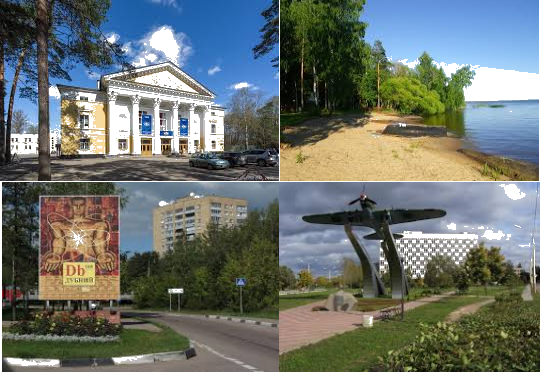
\includegraphics[scale=0.45]{dubna.png}}{}
%\addtobeamertemplate{title page}{\centering 
\includegraphics[scale=0.095]{wpcf2018_2.png}}{}

\title[\bf NICA, introduction lecture]{\textbf{\large {Nuclotron Based Ion Collider fAcility (NICA)}, introduction lecture}}

%\author[P.~Batyuk]{\textit{\textbf{{\footnotesize \underline{P.~Batyuk}, L.~Malinina (SINP MSU, JINR), \\ O.~Rogachevskiy (JINR)}}} \\
%  on behalf of the MPD collaboration}
\author[\bf P.~Batyuk]{\textbf{{\footnotesize P.~Batyuk, pavel.batyuk@jinr.ru}}} 
%on behalf of the MPD collaboration} 
\institute{\bf VBLHEP, Joint Institute for Nuclear Research}
\date{}
% \newpage \footnotesize April 14, 2016}}

\lstset{
  %    frame=tb, % draw a frame at the top and bottom of the code block
  tabsize=4, % tab space width
  showstringspaces=false, % don't mark spaces in strings
  %   numbers=left, % display line numbers on the left
  commentstyle=\color{blue}, % comment color
  keywordstyle=\color{blue}, % keyword color
  stringstyle=\color{red} % string color
}

\begin{document}
\maketitle
\note{Hello,
  First of all, many thanks to organizers of the Workshop!
  I am presenting here Joint Institute for Nuclear Research.
  My talk is related to one of the flagship projects to be realized in the Institute.
  The project is called Nuclotron Based Ion Collider fAcility (NICA).}

\begin{frame}
  \bf
  \frametitle{NICA Complex}
  \vskip -.75cm
  \begin{columns}[t]
    \column{.49\textwidth}
            {\footnotesize
    \begin{block}{}
      \begin{figure}[H]
        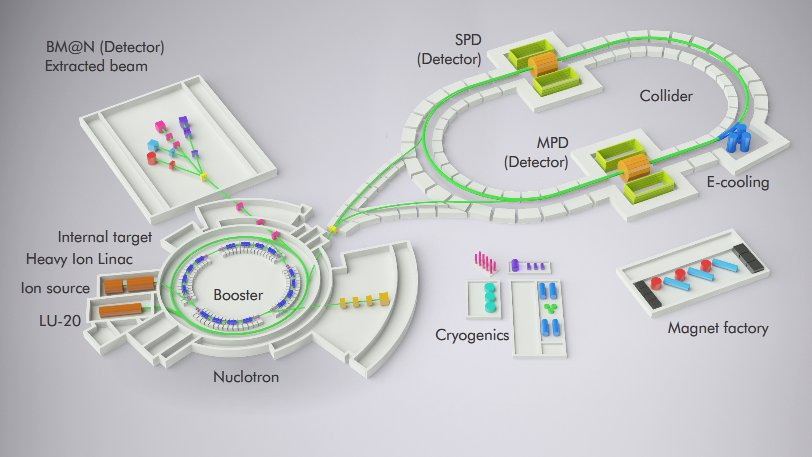
\includegraphics[width=1.\linewidth]{nica_complex1.png}
      \end{figure}
      %\centering The general contractor is  {\color{red} STRABAG} (Bodostal-3 \& PCJ are the sub-contractors)
    %\end{block}
    \vskip -.6cm

   % \begin{block}{}
      \begin{itemize}
      \item Set of accelerators providing particle beams for fixed target and collider experiments
      \item Experimental facilities
      \item Line for assembling and cryogenic testing of SC-magnets
      \item Workshops for construction of the detector elements
      \item NICA innovation center
      \end{itemize}
    \end{block}
        }
            \column{.49\textwidth}
            {\footnotesize 
 \begin{block}{}
      \centering  Beams - {\color{red}$p$, $d$ ... $^{197}Au^{79+}$} \\
      \centering  Collision energy: \\
        $\sqrt{s_{NN}}$ = {\color{red} 4 - 11} GeV
        $E_{lab}$ =  {\color{red}1 - 6} AGeV \\
      Luminosity: {\color{red}$10^{27}~cm^{-2}s^{-1}$} (Au), {\color{red}$10^{32}$}~(p) \\
 \end{block}
 \vskip -.3cm
 \begin{block}{}
      \begin{itemize}
      \item 2 interaction points - {\color{red}MPD} and  {\color{red}SPD}
      \item Fixed target experiment -  {\color{red}BM@N}
      \end{itemize}
 \end{block}
 \vskip -.3cm
 \begin{block}{}
      \begin{itemize}
      \item {\color{red} 2018:} extracted beams of heavy ions (Ar, Kr) are available within the BM@N experiment
      \item {\color{red} 2020-2021}: a first configuration of the MPD setup available.
      \item {\color{red} 2023}: commissioning of the fully designed NICA-complex is foreseen.	
      \end{itemize}
 \end{block}
 }
  \end{columns}
  \note{The NICA complex is being built in Dubna and is considered as a set of different accelerators
    to provide a beam to be used in fixed-target and collider experiments.
    Also, one of the main components of the complex is a line for assembling and cryogenic testing of
    superconducting magnets. It will provide different beam species up to gold ions in energy range
    $\sqrt{s_{NN}}$ = {\color{red} 4 - 11} GeV with a planned level of luminosity of order of $10^{27}~cm^{-2}s^{-1}$ for gold ions.
    The complex will have two points where two experiments will be located: MPD and SPD. Fixed-target program is in
    an active progress and is presented by BM@N experiment.}
\end{frame}

\begin{frame}
  \frametitle{\bf \centering Nuclotron (in operation since 1993)}
  \vskip -.75cm
  \begin{columns}[t]
    \column{.49\textwidth}
    \begin{block}{\bf \centering Modernized in 2010 - 2015}
      \bf 
      \resizebox{\columnwidth}{!}{%
        \begin{tabular}{| l | l |}
          \hline			
          Parameters & Nuclotron \\
          \hline
          type & SC synchrotron \\
          \hline 
          particles & $\uparrow$p, $\uparrow$d, nuclei \\
          \hline
          injection energy [MeV/u] & 5 ($\uparrow$p, $\uparrow$d), 570-685 (Au) \\
          \hline max. kin. energy [GeV/u] & 12.07 ($\uparrow$p), 5.62 ($\uparrow$d), 4.38 (Au) \\
          \hline
          magnetic rigidity [T $\cdot$ m] & 25 - 43.25 \\
          \hline
          circumference [m] & 251.52 \\
          \hline
          cycle for collider mode [s] & 1.5-4.2 (active), 5.0 (total) \\
          \hline
          vacuum [Torr] & $10^{-9}$ \\
          \hline
          intensity, Au [ions/pulse] & 1 $\cdot 10^{9}$ \\
          \hline
          % transition energy [GeV/u] & 7.0 \\
          %  \hline
          spill of slow extraction [s] & up to 10 \\
          \hline
        \end{tabular}
      }
    \end{block}
     \vskip -.3cm
    {\bf
    \begin{block}{}
      \begin{itemize}
      \item The project approved in {\color{red} 1986}
      \item Commissioning \& first beam, {\color{red} March 1993}
      \item Slow extraction in {\color{red} 2000}
      \end{itemize}
     % \vskip .6cm
      \begin{center}
        Ions from p to Xe \\
        (C, Mg, Fe, Ar, Kr) \\
        Polarized p \& d beams
      \end{center}
    \end{block}
    }
    
    \column{.49\textwidth}
    \begin{block}{}
      \begin{figure}[H]
        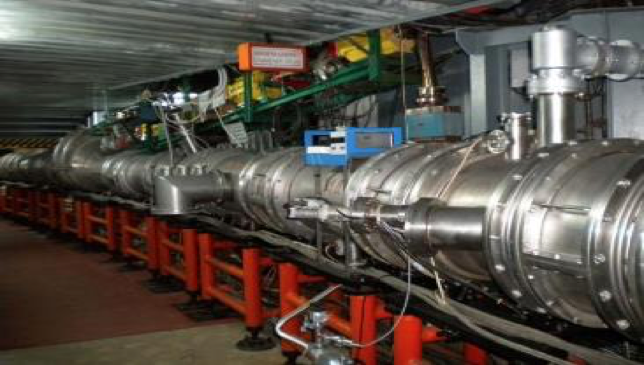
\includegraphics[width=1.\linewidth]{nuclotron1.png} \\
        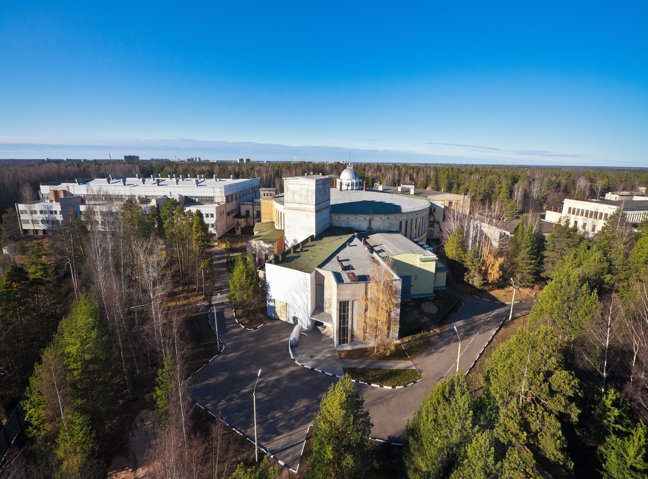
\includegraphics[width=1.\linewidth]{nuclotron2.png}
      \end{figure}
    \end{block}
  \end{columns}
  \note{The Nuclotron as a main accelerator of the complex is a synchrotron based on the SC magnets developed at JINR,
    was put in operation in 1993. In was essentially modernized in 2010-2015. It will provide acceleration of gold ions up to
    kinetic energy 4.4 GeV/u, and protons up to 12 GeV. In February we had an experimental run aimed at realizing
    fixed-target program within the BM@N experiment.}
\end{frame}

\begin{frame}
  \frametitle{\bf \centering Nuclotron}
   \vskip -.75cm
  \begin{columns}[t]
    \column{.47\textwidth}
    \begin{block}{\bf \centering Run № 53, 1450 h, the longest one}
      \begin{figure}[H]
        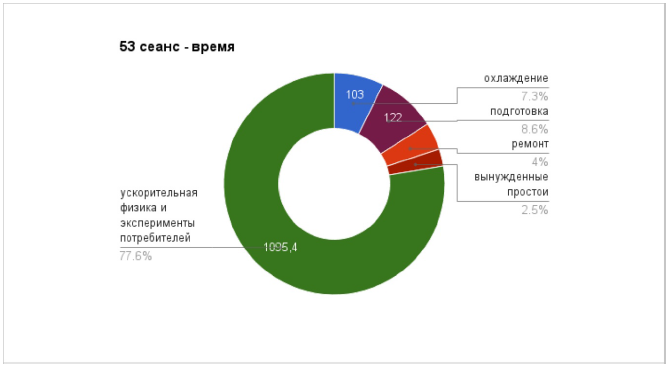
\includegraphics[width=1.\linewidth]{run53.png}
      \end{figure}
    \end{block}
    \vskip -0.2cm
    {\footnotesize 
    \begin{block}{}
      \begin{itemize}
      \item {\bf {\color{red} Run53} - Polarized, unpolarized deuterons, maximum energy of extracted beam 4.6 GeV/u}
      \item {\bf {\color{red} Run54} - Carbon beam}
      \item {\bf {\color{red} Run55} - Argon \& Krypton beams}
      \end{itemize}
    \end{block}
    }
    \column{.47\textwidth}
     \begin{block}{\bf \centering Run № 54, 1150 h}
       \begin{figure}[H]
         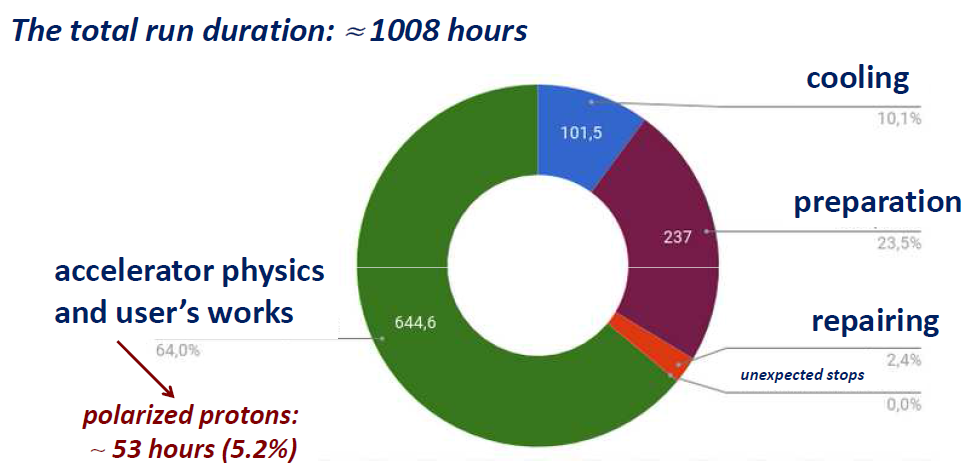
\includegraphics[width=1.\linewidth]{run54.png}
       \end{figure}
     \end{block}
      \begin{block}{\bf \centering Run55: Feb - Apr, 2018}
      \begin{figure}[H]
        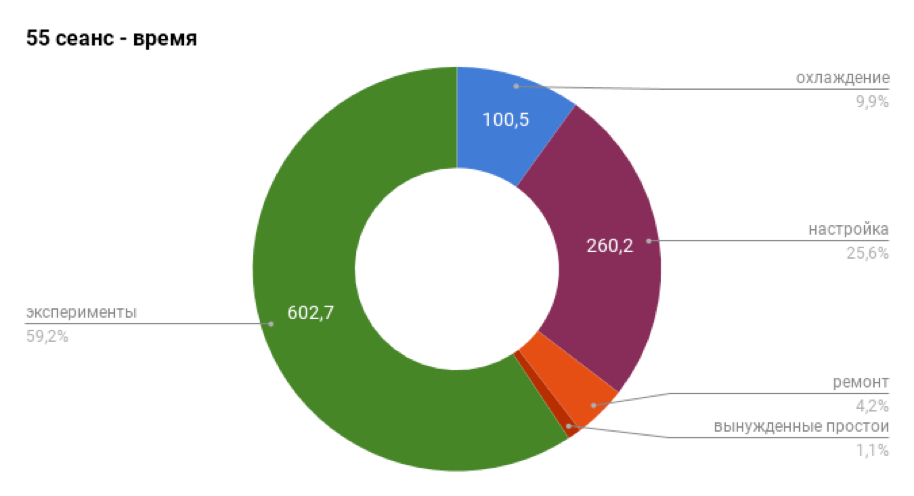
\includegraphics[width=1.\linewidth]{run55.png} \\
      \end{figure}
    \end{block}    
  \end{columns}  
\end{frame}

\begin{frame}
  \frametitle{\bf \centering Booster}
  \vskip -.75cm
  \begin{columns}[t]
    \column{.53\textwidth}
    \begin{block}{\bf \centering {\small Commissioning started in 2018}}
      \bf
      \resizebox{\columnwidth}{!}{%
        \begin{tabular}{| c | c |}
          \hline	
          Parameter & Booster \\
          \hline
          type & SC synchrotron \\
          \hline
          particles & ions $A/Z \leq 3$ \\
          \hline
          injection energy [MeV/u] & 3.2 \\
          \hline
          maximum energy [MeV/u] & 600 \\
          \hline
          magnetic rigidity [T $\cdot$ m] & 1.6 - 25.0 \\
          \hline
          circumference [m] & 210.96 \\
          \hline
          vacuum [Torr] & $10^{-11}$ \\
          \hline
          intensity [Au ions/pulse] & $1.5 \cdot 10^{9}$ \\
          \hline
          RF range [MHz] & 0.5 - 2.53 \\
          \hline
        \end{tabular}
      }
      \vskip -.3cm
      \begin{figure}[H]
        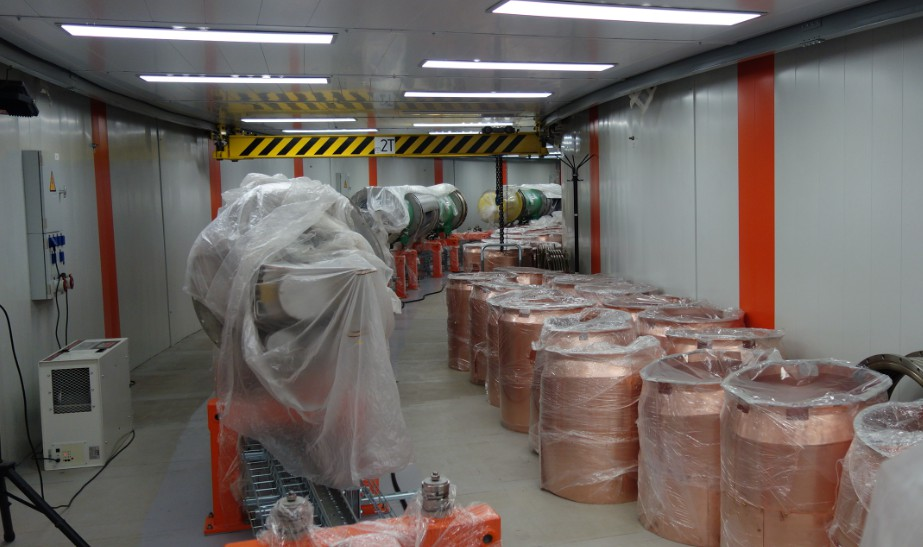
\includegraphics[width=1.\linewidth]{booster_tunnel2_2019.jpg} 
      \end{figure}
    \end{block}
    %\begin{block}{\bf \centering {\small RF stations are tested}}
    %\begin{figure}[H]
    %  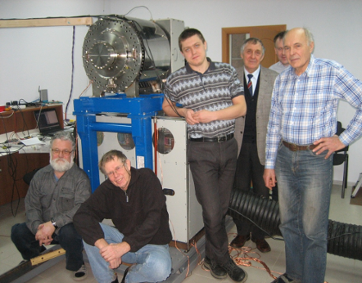
\includegraphics[width=1.\linewidth]{booster3.png} 
    %\end{figure}
    %\end{block}

    \column{.4\textwidth}
    \begin{block}{\bf \centering {\small Tunnel for Booster}}
      \begin{figure}[H]
        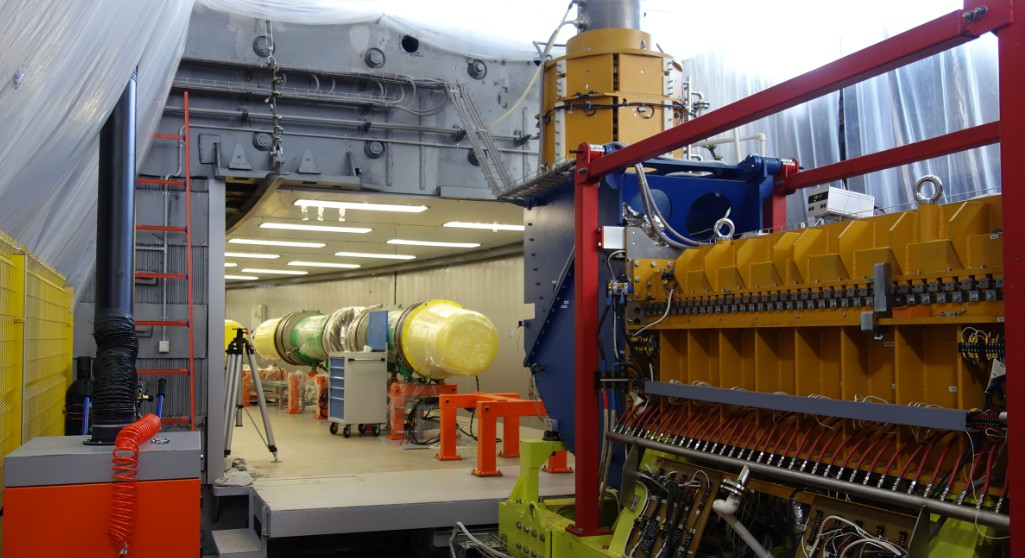
\includegraphics[width=1.\linewidth]{booster_tunnel_2019.jpg} 
      \end{figure}
    \end{block}
    \vskip -.3cm
    %\begin{block}{\bf \centering {\small Electron Cooling System}}
    %  \begin{figure}[H]
    %    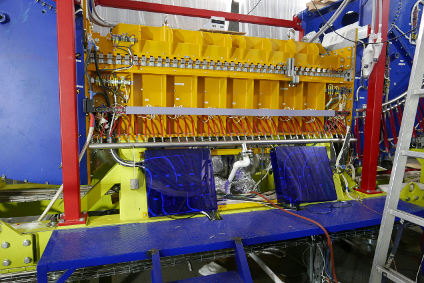
\includegraphics[width=1.\linewidth]{booster2.png}
    %  \end{figure}
    %\end{block}
    {\scriptsize \bf 
    \begin{block}{}
      \begin{itemize}
        \item Fabrication of the magnetic system is completed.
        \item Start of assembly - September 2018.
        \item First (technological) run - end of 2019.
        \item Commissioning - end of 2020        
      \end{itemize}
      {\color{red} First magnet was installed on 19 September 2018!}
    \end{block}
    }
  \end{columns}
  \note{The Booster should accelerate ions  up to 600 MeV per nucleon with A/Z ratio less or equal to 3.
    The magnetic ring with circumference of 211 m is located inside the window of the Synchrophasotron yoke.
    The Synchrophasotron was disassembled in 2002. To provide the required beam quality the Booster is equipped with electron
    cooling system.}
\end{frame}

\begin{frame}
  \bf
  \frametitle{\bf \centering \footnotesize Line for assembling and cryogenic testing of SC-magnets}
  \vskip -.4cm
  \begin{columns}[c]
    \column{.53\textwidth}
    \begin{block}{\bf \centering Main production areas:}
      %\vskip -.15cm
      \begin{itemize}
      \item Incoming inspection zone
      \item SC cable production hall
      \item SC coils production hall
      \item Area for assembling the magnets
      \item Area for the magnetic measurements under the room temperature
      \item Leakage test area
      \item Area for mounting the SC-magnets inside cryostats
      \item Cryogenic tests bench
      \end{itemize}   
    \end{block}
    \vskip -0.35cm
    \begin{block}{}
      {\color{red} All of the Booster magnets are produced \& tested}
    \end{block}
    
    \column{.41\textwidth}
    \begin{block}{}
      \begin{figure}[H]
        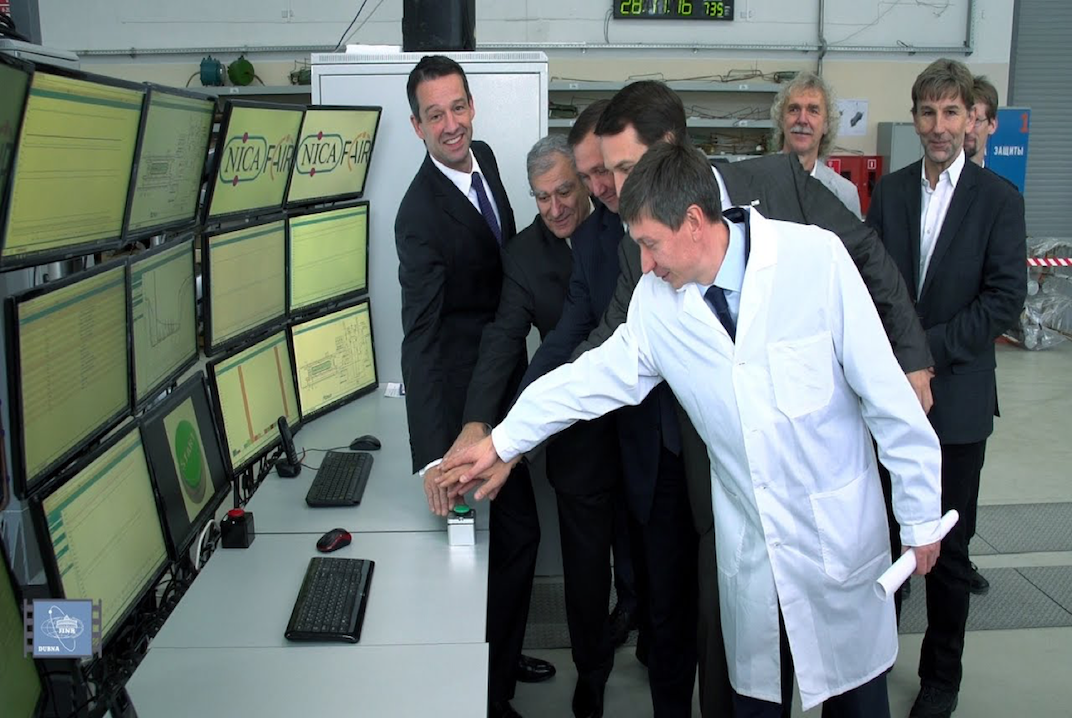
\includegraphics[width=1.\linewidth]{SC_magnetLine.png} \\
        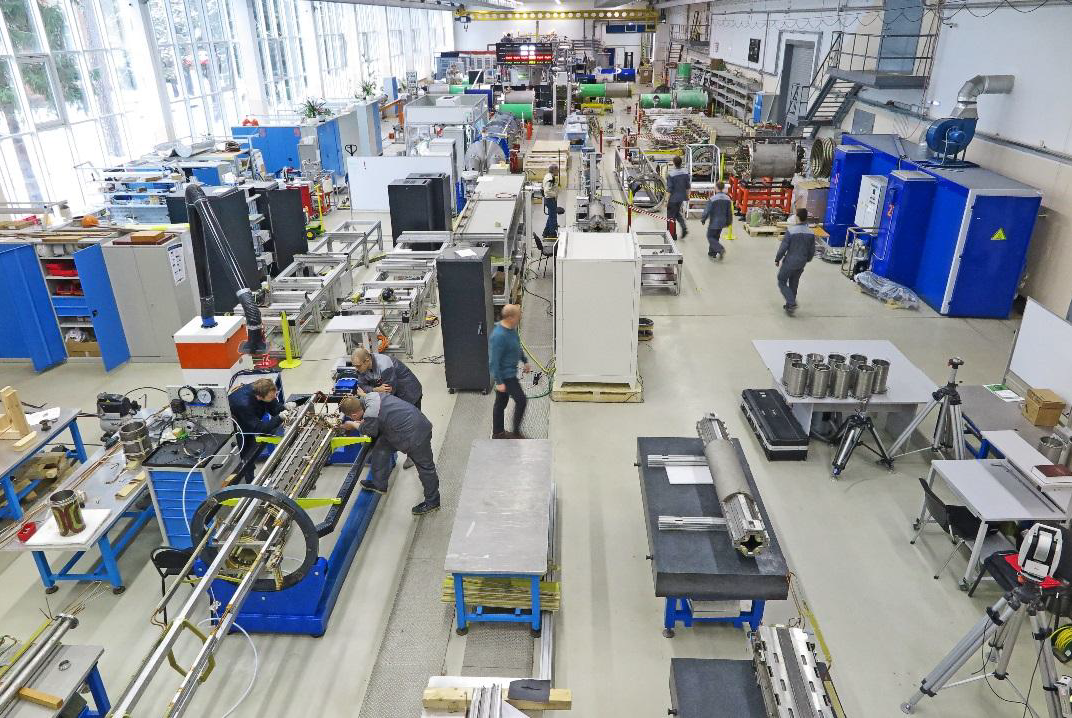
\includegraphics[width=1.\linewidth]{SC_assemblingHall.png}
      \end{figure}
    \end{block}
    \vskip -.3cm
    \begin{block}{}
      {\footnotesize \color{Red} \bf \centering 450 magnets for NICA and FAIR projects}
    \end{block}
  \end{columns}
  \note{Line for assembling and cryogenic testing of SC-magnets includes is full and includes different production areas.
    Among them one can separate superconducting cable production, area for assembling magnets, area for magnetic measurements
    at root temperature, leakage test area and other ones.}
\end{frame}

\begin{frame}
  \frametitle{\bf \centering KRION 6T - heavy ion source}
  \begin{columns}[c]
    \column{.125\textwidth}   
    \column{.75\textwidth}
    \begin{block}{\bf \centering Used during Nuclotron RUN №55}
      \begin{figure}[H]
        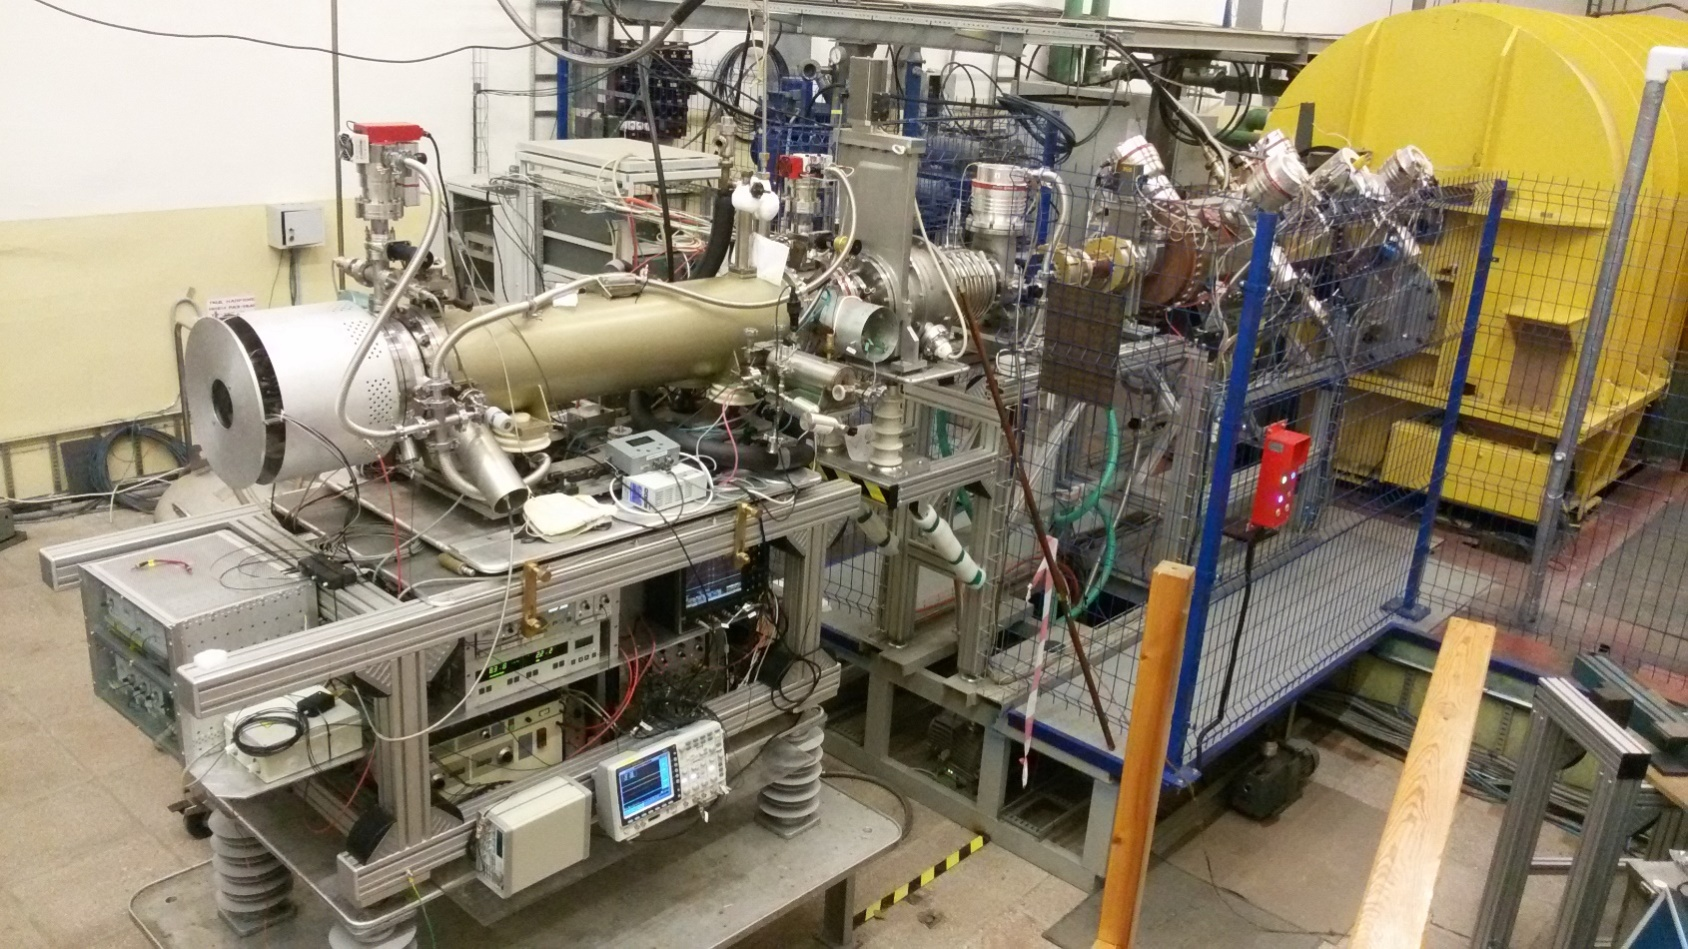
\includegraphics[width=1.\linewidth]{krion6T.jpg} 
      \end{figure}
    \end{block}
    \column{.125\textwidth}
      \end{columns}
    {\bf 
    \begin{block}{}
      \begin{itemize}
      \item Cryogenic heavy ion source KRION - Electron String Ion Source (ESIS) -
        provides up to $2.5 \cdot 10^{9}$ $Au^{31+}$ ion / cycle at repetition frequency up to 10 Hz
      \end{itemize}
    \end{block}
    } 
\end{frame}

\begin{frame}
  \frametitle{\bf \centering Linacs}
  \vskip -.75cm
  \begin{columns}[t]
    \column{.44\textwidth}
    \begin{block}{\bf \centering LU-20}
      \begin{figure}[H]
        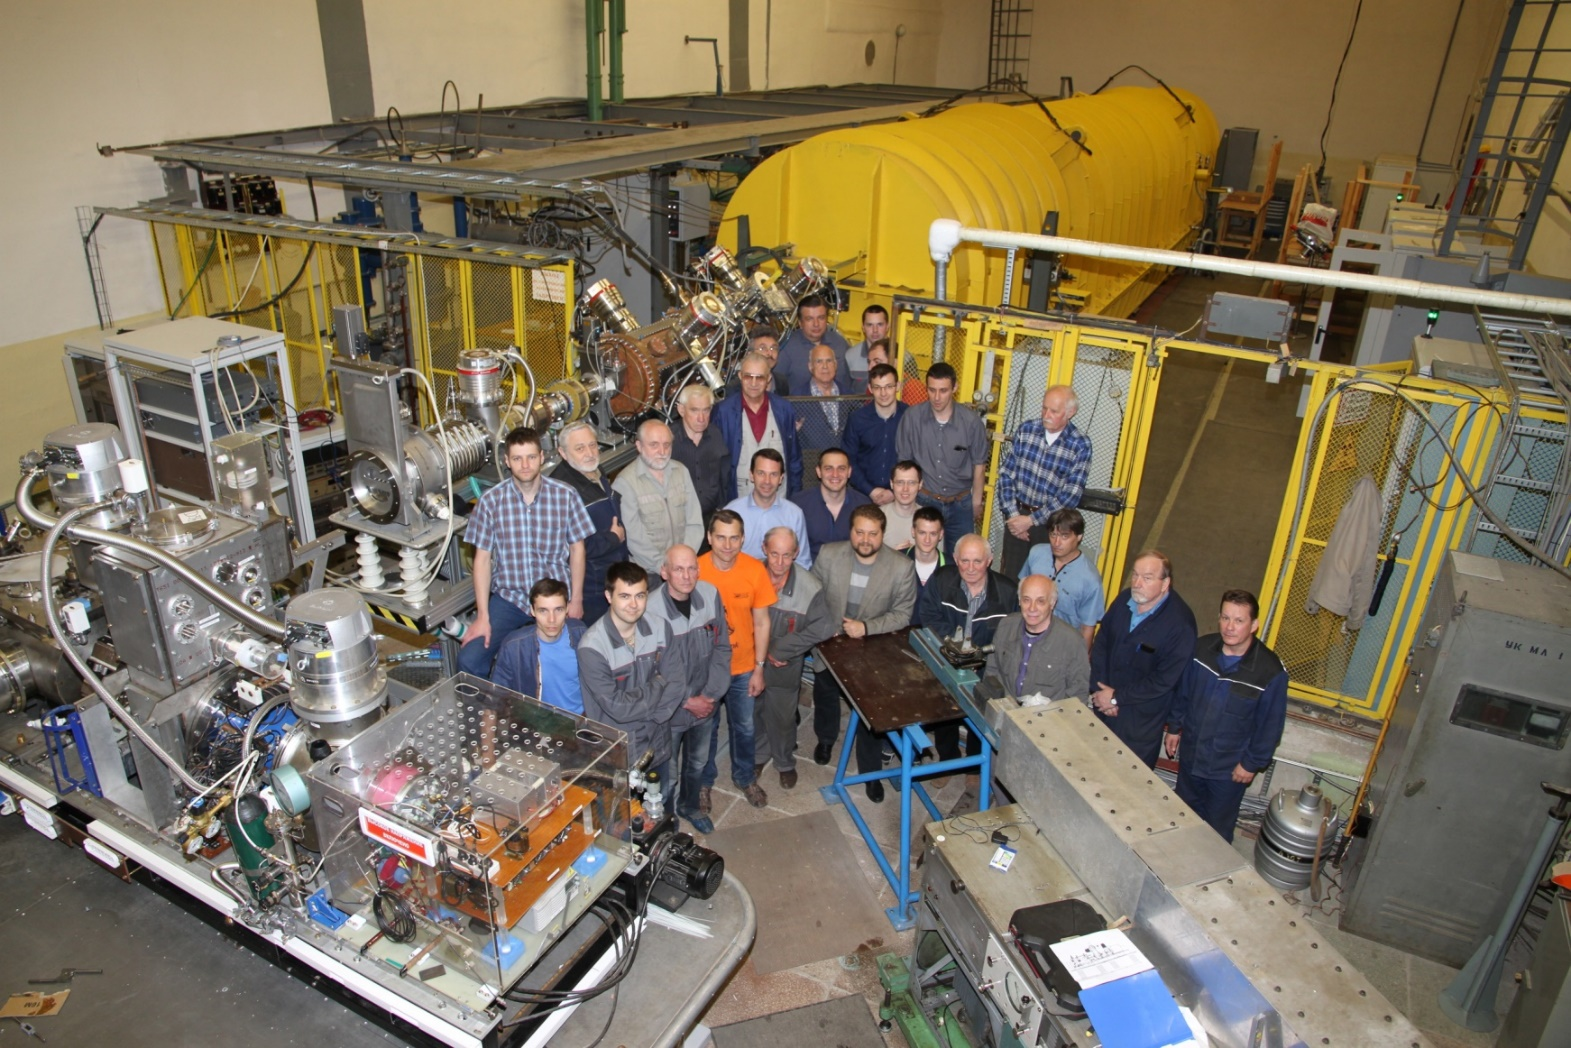
\includegraphics[width=1.\linewidth]{lu20.jpg} 
      \end{figure}
    \end{block}
    
    \column{.52\textwidth}
    \begin{block}{\bf \centering HILAC}
      \begin{figure}[H]
        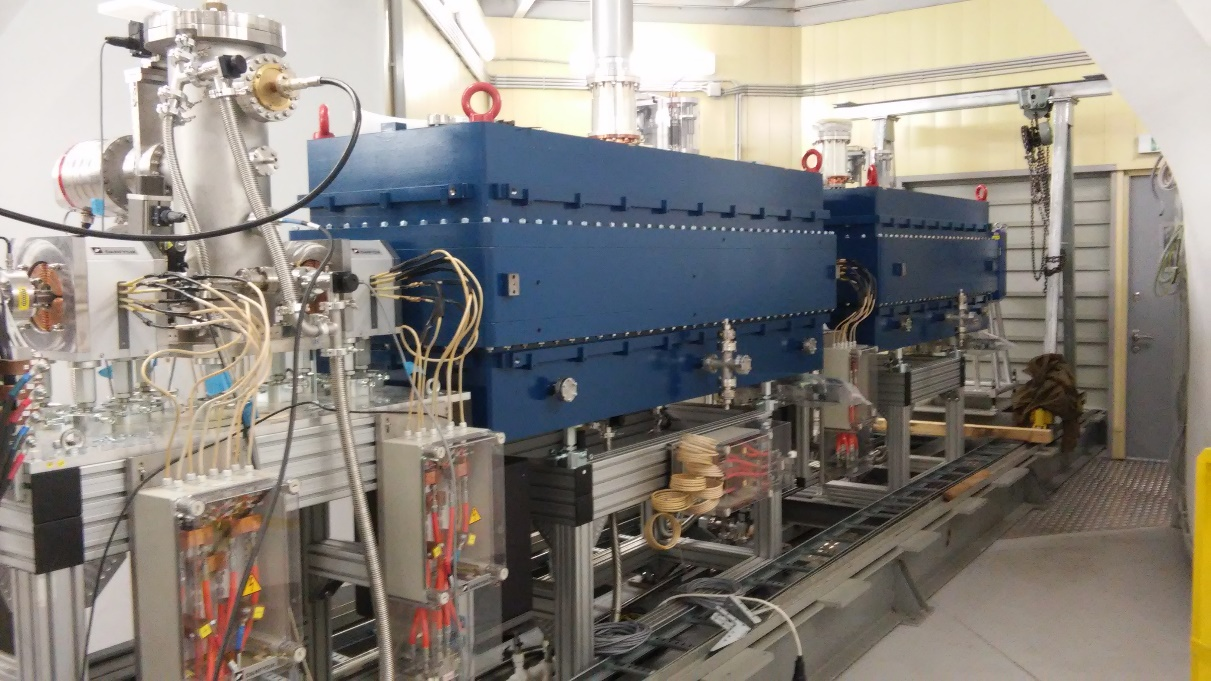
\includegraphics[width=1.\linewidth]{hilac.jpg} 
      \end{figure}
    \end{block}
       
  \end{columns}
   {\bf \footnotesize 
     \begin{block}{}
       \begin{center}
            \begin{itemize}
            \item {\color{red} LU-20} - JINR, INR, ITEP, MEPhI (Commissioning - {\color{blue} May 2016})
            \item {\color{red} HILAC} - BEVATECH OHG (Commissioning - {\color{blue} October 2018})
            \end{itemize}
       \end{center}
          \end{block}
        }
    \begin{block}{}
       \bf
      \resizebox{\columnwidth}{!}{%
        \begin{tabular}{| c | c | c |}
          \hline	
           & LU-20 & HILAC ({\color{red} NEW!}) \\
          \hline
          Mass to charge ratio $A / Z$ & 1-3 & 1-6 \\
          \hline
          Injection energy [keV / a.m.u.] & 150 for A/Z 1-3 & 17 \\
          \hline
          Extraction energy [MeV / a.m.u.] & 5 (A/Z 1-3) & 3.24 (A/Z = 6) \\
          \hline
        \end{tabular}
      }
    \end{block}
\end{frame}

\begin{frame}
  \frametitle{\bf \centering Collider as the main ingredient of the kitchen:)}
  \vskip -0.75cm
  \begin{columns}[t]
    \column{.15\textwidth}
    
    \column{.7\textwidth}
     \begin{block}{\bf \centering Collider construction: Official start up of the construction is {\color{red} 25 March 2016}}
      \begin{figure}[H]
        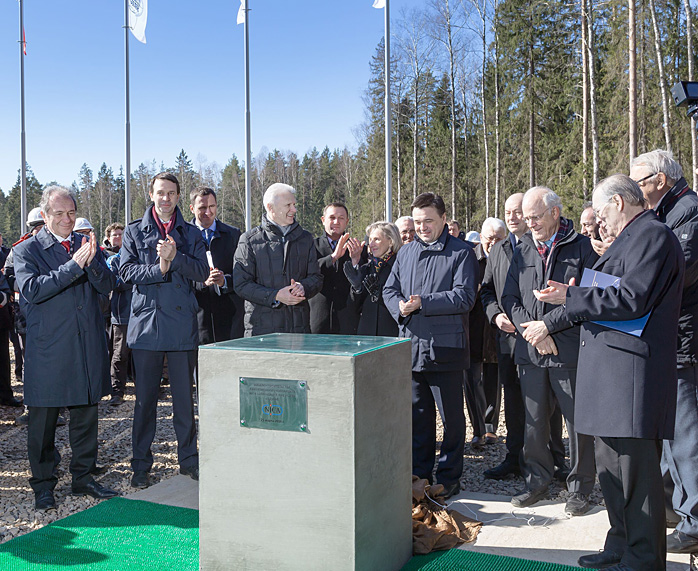
\includegraphics[width=1.\linewidth]{collider_start.jpg} 
      \end{figure}
     \end{block}

     \column{.15\textwidth}
     
  \end{columns}
\end{frame}

\begin{frame}
  \bf
  \frametitle{\bf \centering Collider}
  \vskip -.25cm
  \begin{block}{}
     \centering \url{http://nucloweb.jinr.ru/nucloserv/205corp.htm}
  \end{block}
  \vskip -.66cm
  \begin{columns}[t]
    \column{.49\textwidth}
   % \begin{block}{\bf \centering NICA site online \\ \url{http://nucloweb.jinr.ru/nucloserv/205corp.htm}}
    \begin{block}{}
    \begin{figure}[H]
        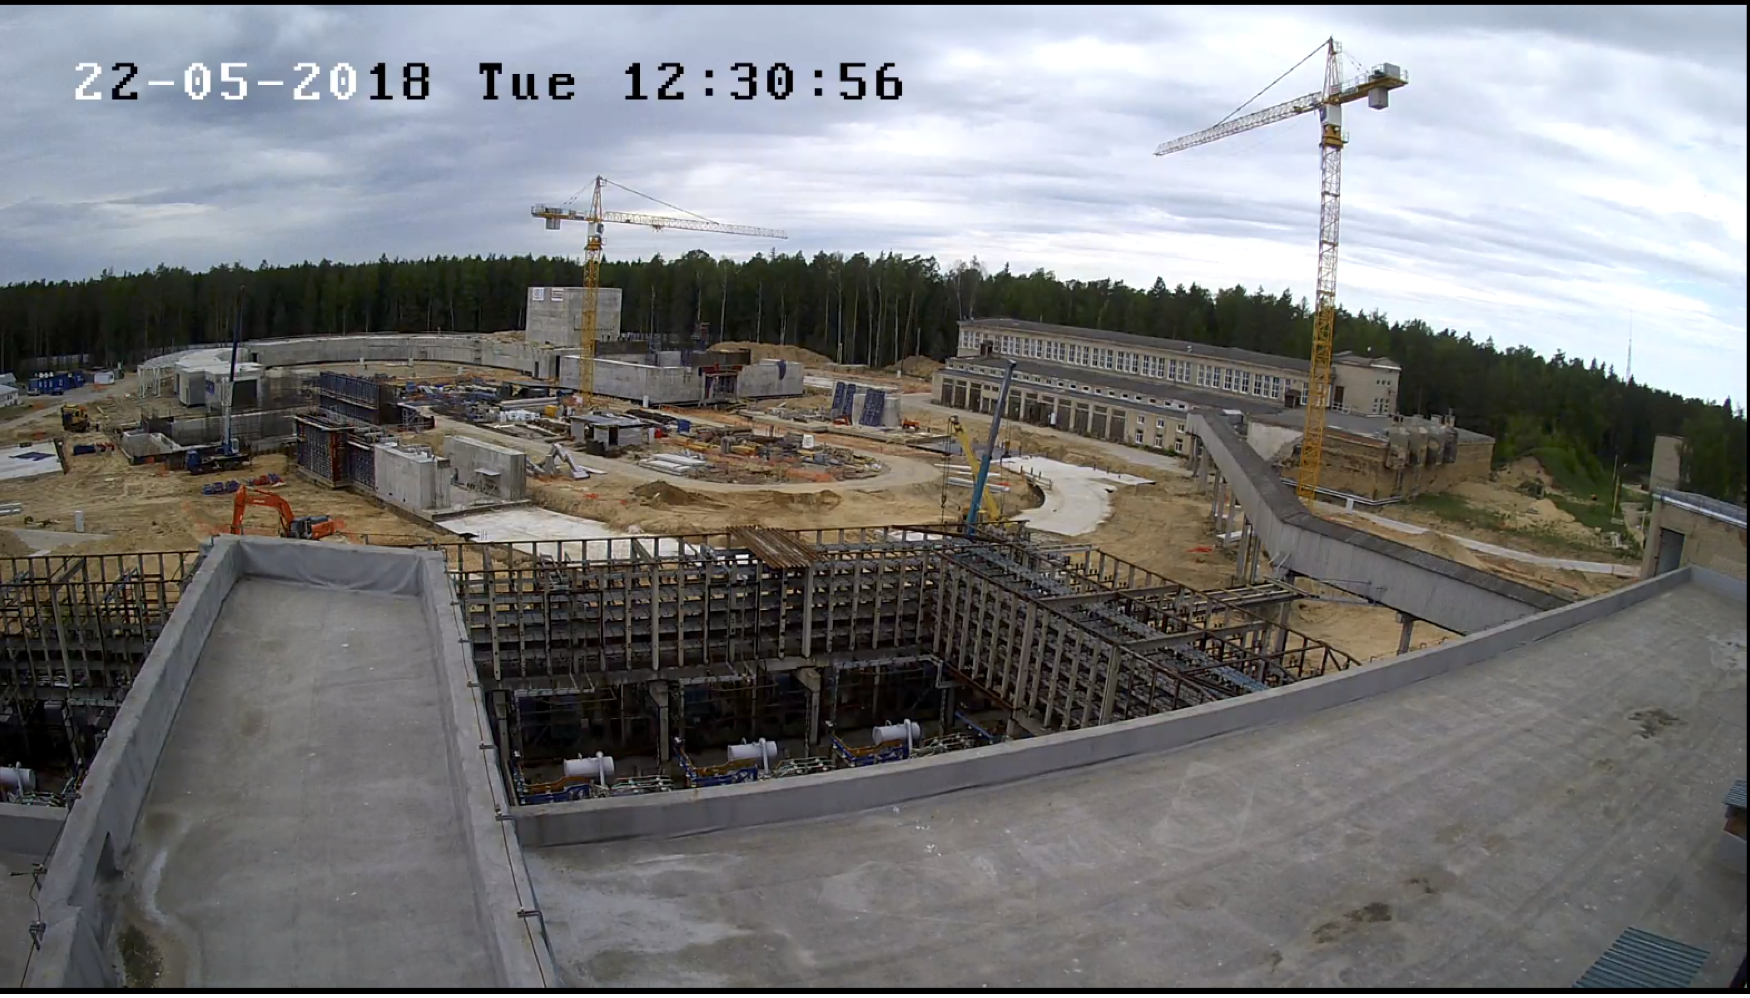
\includegraphics[width=1.\linewidth]{collider_online.png}
        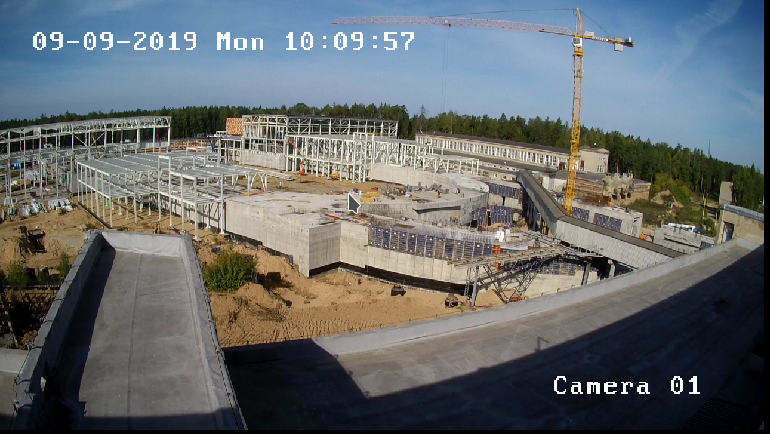
\includegraphics[width=1.\linewidth]{Screenshot_20190909_101022.png}
      \end{figure}
    \end{block}
    %\begin{block}{}

    %\end{block}
    \column{.49\textwidth}
    \begin{block}{}
      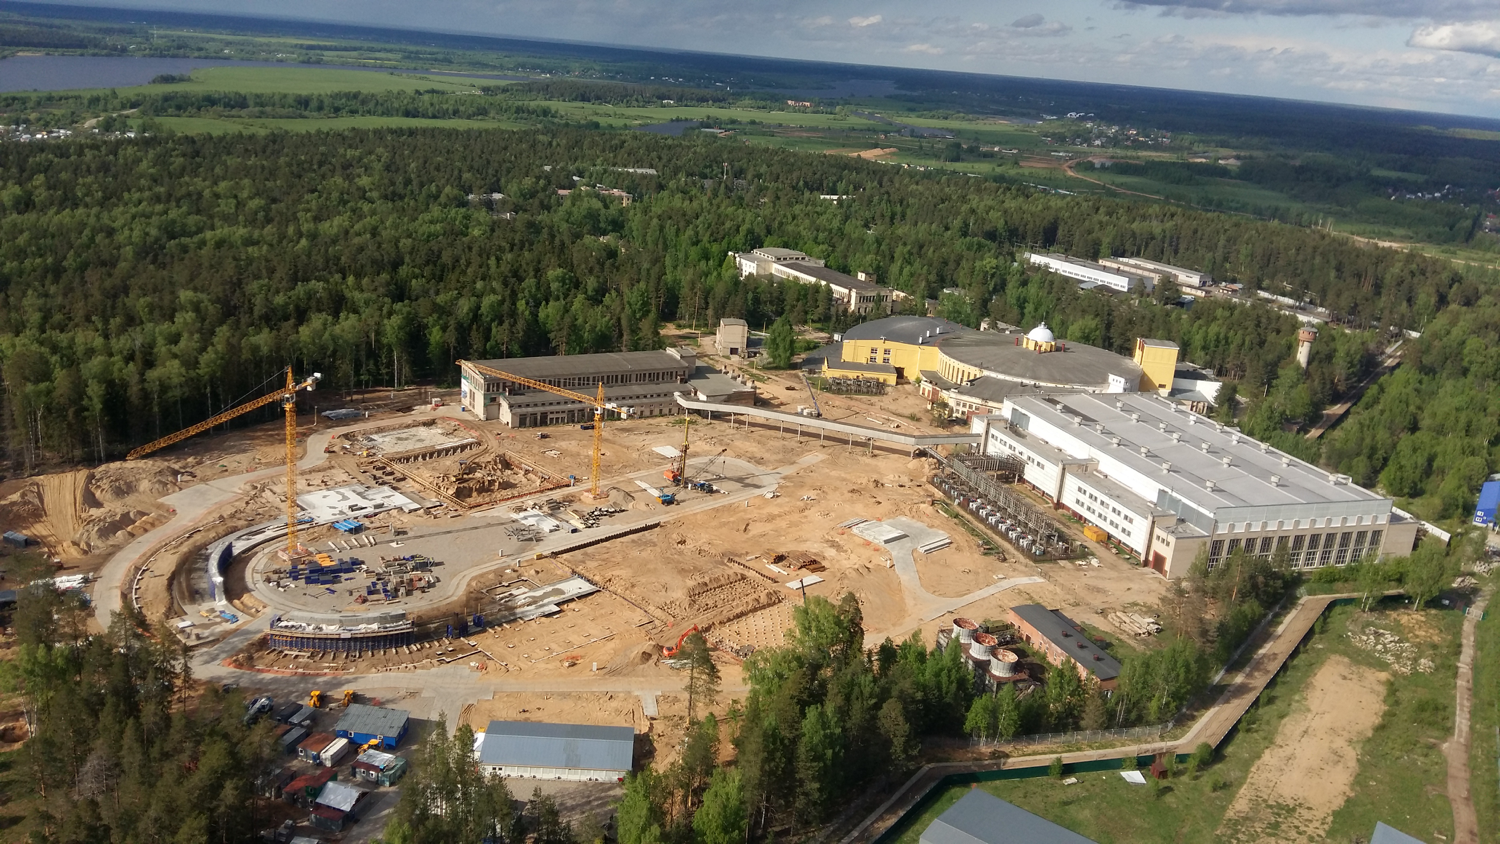
\includegraphics[width=1.\linewidth]{NICA_collider_panPhoto.png}
    \end{block}
    \vskip -.3cm
    \begin{block}{\bf \centering Technical params:}
      \resizebox{\columnwidth}{!}{%
        \begin{tabular}{| c | c |}
          \hline
          Ring circumference [m] & {\color{Red} 503.04} \\
          \hline
          Number of bunches & 22 \\
          \hline
          $\Delta_{bunch~length}$ [m] & 0.6 \\
          \hline
          Max. energy $\sqrt{s_{NN}}$ [GeV] & {\color{Red} 11} \\
          \hline
          $\Delta p / p$ $[10^{-3}]$ & 1.6 \\
          \hline
          Luminosity [$cm^{-2} \cdot s^{-1}$] & {\color {Red} $10^{27}$} \\
          \hline
        \end{tabular}
        }

    \end{block}
  \end{columns}
  \note{The lattice design and prototyping of most collider elements are completed. The ring circumference is two time larger
    than the Nuclotron one. For the gold beam a luminosity at the energy above 10 GeV per nucleon will be of order of $10^{27}$}
\end{frame}

\begin{frame}
  \frametitle{\bf \centering Collider}
  \begin{block}{\bf \centering September 2018}
     \begin{figure}[H]
        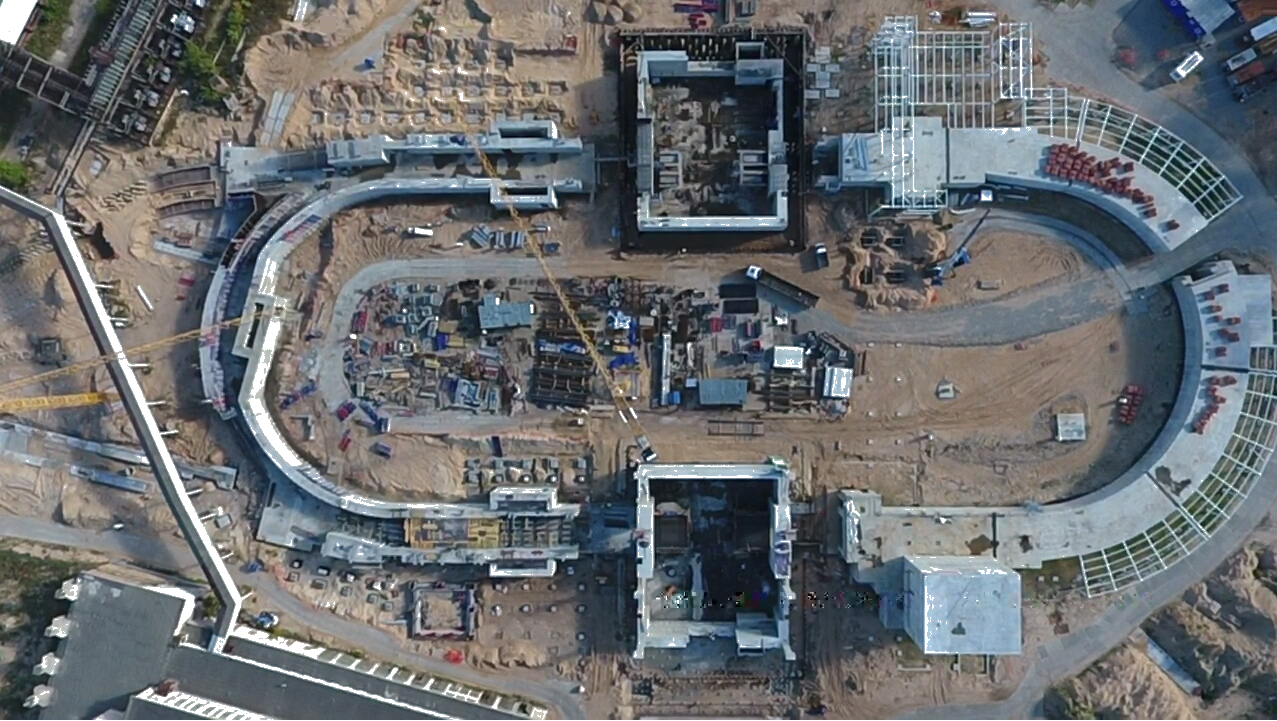
\includegraphics[width=.8\linewidth]{collider_now.png} 
      \end{figure}
  \end{block}
\end{frame}

\begin{frame}
  \frametitle{\bf \centering Collider}
  \begin{block}{\bf \centering August 2019}
     \begin{figure}[H]
        \includegraphics[width=.8\linewidth]{collider_August2019.png} 
      \end{figure}
  \end{block}
\end{frame}

\begin{frame}
  \frametitle{\bf \centering Cryogenic facility}
  \vskip -0.75cm
  \begin{columns}[t]
    \column{.15\textwidth}
     \column{.85\textwidth}
    \begin{block}{\bf \centering New helium liquefier (1000 L/H)}
      \begin{figure}[H]
        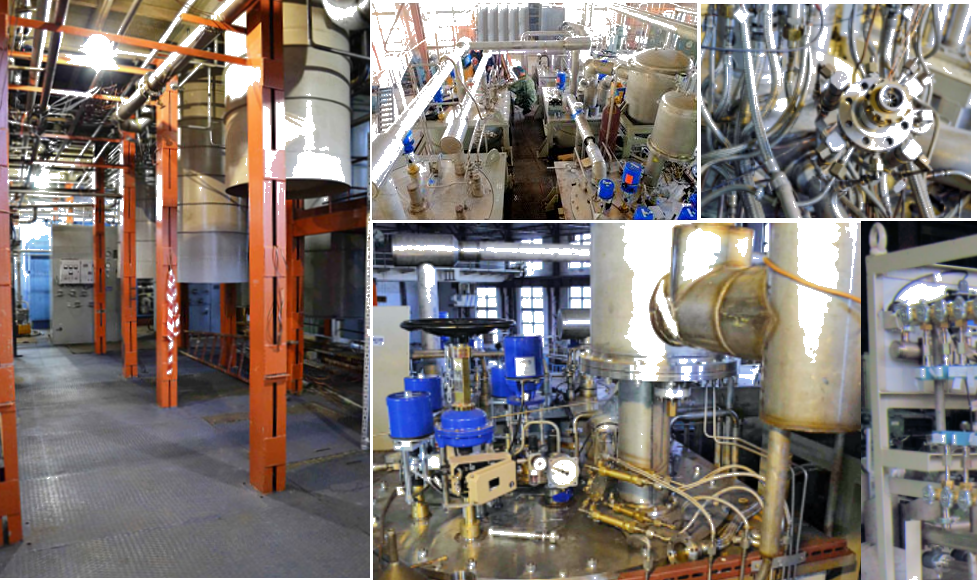
\includegraphics[width=1.\linewidth]{liquefier.png} 
      \end{figure}
    \end{block}
    \column{.15\textwidth}
    
  \end{columns}
  \begin{block}{}
    \bf Finally the cooling power should be doubled from \\ 4 kW to 8 kW @ 4.5K
  \end{block}
\end{frame}

\begin{frame}
  \bf
  \frametitle{\bf \centering QCD phase diagram}
  \vskip -.75cm
  \begin{columns}[t]
    \column{.49\textwidth}
    \begin{block}{}
      \begin{figure}[H]
        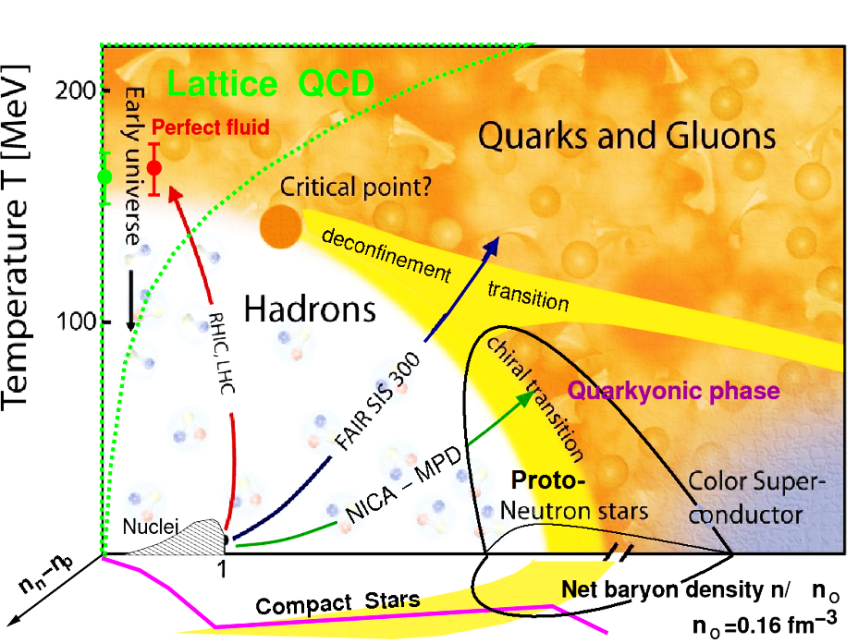
\includegraphics[width=1.\linewidth]{qcd_diagram.png}
      \end{figure}
    \end{block}
    \vskip -.75cm

    \begin{columns}[t]
      \column{.48\textwidth}  
      \begin{block}{\bf \centering {\tiny High energy:}}
        {\tiny
          \begin{itemize}
          \item $N_{baryons} \approx N_{antibaryons}$
          \item Lattice QCD predicts crossover transition between hadronic and partonic matter
          \item ALICE, ATLAS, CMS, STAR, PHENIX
          \end{itemize}
        }
      \end{block}
      \column{.48\textwidth}
      \begin{block}{\bf \centering {\tiny High net-baryon density:}}
        {\tiny
          \begin{itemize}
          \item $N_{baryons} >> N_{antibaryons}$
          \item Lattice QCD not applicable, models predict structures and exotic phases 
          \item BES @ RHIC, NA61, CBM, {\color{red} NICA/MPD, BM@N}
          \end{itemize}
        }
      \end{block}
    \end{columns}

    \column{.48\textwidth}
    \begin{block}{\bf \centering  Landscape of experiments exploring QCD phase diagram}
      \vskip .25cm
      \begin{figure}[H]
        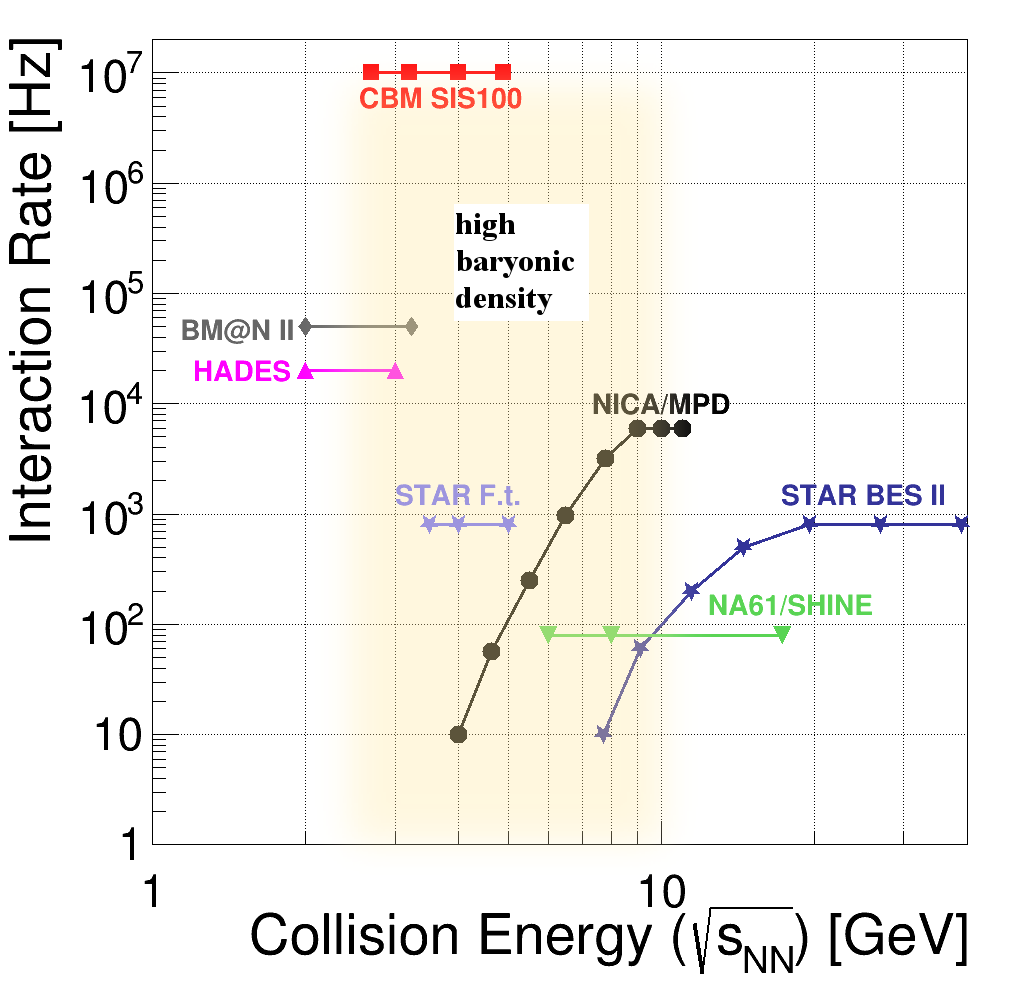
\includegraphics[width=1.\linewidth]{QCD_dense_matter_experiments.png}
      \end{figure}
    \end{block}
  \end{columns}
  \note{One of the most urgent task for the study of the QCD phase diagram is density frontier.
    According to various calculations maximum freeze-out density is reached at the energy range around $\sqrt{s_{NN}}$ = 10 GeV/n.
    So, NICA is well suited for exploring the transition between the hadronic and quark-gluon phases at the high net-baryon
    density. This is the top priority of the NICA program. \\
    The landscape of HIC experiments, present and future, in the energy
    region of max baryonic density are presented in this figure. Among fixed target experiments
    CBM at FAIR will provide maximum interaction rate. There are only two collider experiments – NICA and STAR BES with
    a difference in interaction rate of 3-4 orders of magnitude. Two NICA experiments - BM@N with fixed target and MPD
    at the collider will cover the whole indicated energy region.
  }
\end{frame}

\begin{frame}
  \bf
  \begin{block}{}
    \begin{center}
      {\Huge Experiments in collider mode}
    \end{center}
  \end{block}
\end{frame}

\begin{frame}
  \bf
   \vskip -0.3cm
  \frametitle{\centering \bf {\small MultiPurpose Detector (MPD) for $A + A$ collisions @ NICA}}
  \begin{columns}[t]
    \column{.49\textwidth}
    \vskip -0.5cm
    \begin{block}{\bf \centering MPD Layout:}
      \begin{figure}[H]
        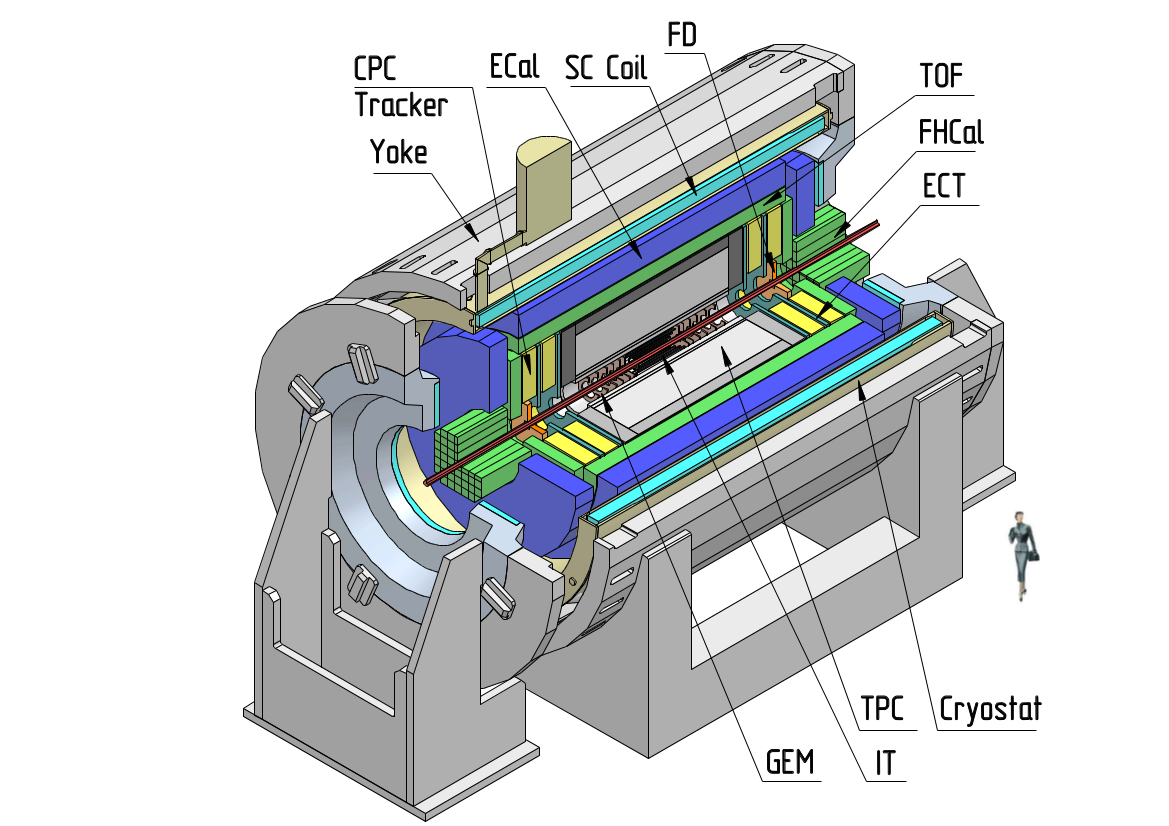
\includegraphics[width=1.\textwidth]{mpd.png} 
      \end{figure}
    \end{block}
    \vskip -0.3cm
           {\tiny 
             \begin{block}{\bf \centering Participants:}           
               \begin{columns}[t]
                 \column{.49\textwidth}
                 \vskip -0.4cm
                 % \vspace -1cm
                 \begin{itemize}
                   %\item JINR, Dubna
                 \item Tsinghua University, Beijing, China
                 \item GSI, Darmstadt, Germany
                 \item WUT, Warsaw, Poland
                 \end{itemize}
                 
                 \column{.49\textwidth}
                 \vskip -0.3cm
                 \begin{itemize}
                 \item MEPhI, Moscow, Russia 
                 \item INR, RAS, Russia
                 \item PPC BSU, Minsk, Belarus
                 \item Dubna, JINR, Russia
                 \end{itemize}           
               \end{columns}
             \end{block}
           }
           
           \column{.49\textwidth}
                  {\tiny
                    \vskip -0.5cm
                    \begin{block}{\bf \centering Benefits:}
                      %               \begin{columns}[t]
                      %                 \column{.23\textwidth}
                      \begin{itemize}
                      \item Hermeticity, $2\pi$-acceptance in azimuth
                      \item 3D-tracking (TPC, ECT)
                      \item Vertex high-resolution (IT)
                        %                \end{itemize}
                        %                \column{.43\textwidth}
                        %                \begin{itemize}
                      \item Powerful PID (TPC, TOF, ECAL)
                        \begin{itemize}
                        \item  {\tiny$\pi, K$ up to 1.5 GeV/c}
                        \item {\tiny$K, p$ up to 3 GeV/c}
                        \item {\tiny$\gamma, e$ from 0.1 GeV/c up to 3 GeV/c}
                        \end{itemize}
                        %                 \end{itemize}
                        %                 \column{.23\textwidth}
                        %                 \begin{itemize}
                      \item Precise event characterization (FHCAL)
                      \item Fast timing and triggering (FFD)
                      \item Low material budget
                      \item High event rate (up to 7 kHz) 
                      \end{itemize}
                      %              \end{columns}
                    \end{block}
                  }
                  \vskip -0.3cm
                  \begin{block}{\bf \centering Realization progress:}
                    %\vskip 0.40cm
                    %  \begin{center}
                    {\scriptsize
                      \begin{itemize}
                        {\tiny \item TDR - completed / close to  completion }
                        {\tiny \item Preparation for / start of mass production} 
                      \item First stage - {\color{red} 2021} (ready for cosmics - end of {\color{red} 2020}) 
                      \item Second stage and full commissioning (IT + end-cups) - {\color{red} 2023}
                      \end{itemize}
                    }
                    %  \end{center}
                    
                  \end{block}
  \end{columns}
  \note{The MPD will be the first detector operated at the Collider. Main target is a study of hot and dense baryonic matter
    at the energy range of maximum net-baryonic density.
    The MPD will be put in operation by two stages.
    At the first stage the barrel part will be equipped with major tracking detectors like TPC, TOF end ECAL.
    FHCAL and FD will be operational as well.
    At the second stage the detector will be supplemented with IT and end-cap subdetectors.
  }
\end{frame}

\begin{frame}
  \frametitle {\bf \centering Assembling MPD ...}
  \vskip -0.5cm
  \begin{columns}[t]
     \column{.075\textwidth}
    \column{.85\textwidth}
   \begin{block}{}
       \begin{figure}[H]
         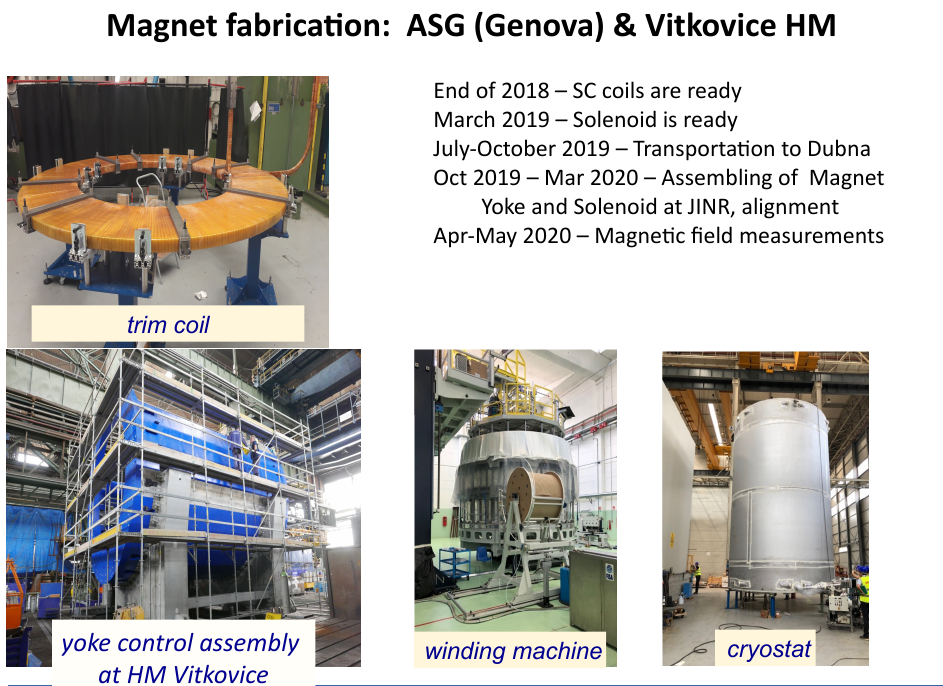
\includegraphics[width=1.\textwidth]{MPD_magnetFabrication.png}
       \end{figure}
   \end{block}
     \column{.075\textwidth}
  \end{columns}
\end{frame}

\begin{frame}
  \frametitle {\bf \centering Assembling MPD ...}
   \vskip -0.5cm
  \begin{columns}[t]
     \column{.075\textwidth}
    \column{.85\textwidth}
   \begin{block}{}
       \begin{figure}[H]
         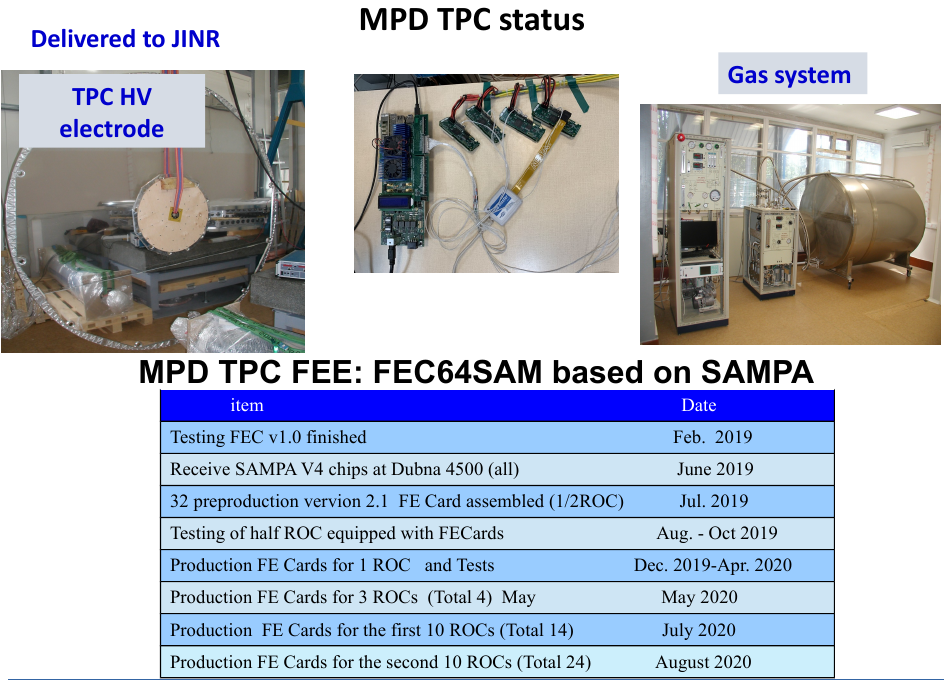
\includegraphics[width=1.\textwidth]{MPD_tpcFabrication.png}
       \end{figure}
   \end{block}
     \column{.075\textwidth}
  \end{columns}
\end{frame}

\begin{frame}
  \frametitle {\bf \centering Assembling MPD ...}
   \vskip -0.5cm
  \begin{columns}[t]
     \column{.075\textwidth}
    \column{.85\textwidth}
   \begin{block}{}
       \begin{figure}[H]
         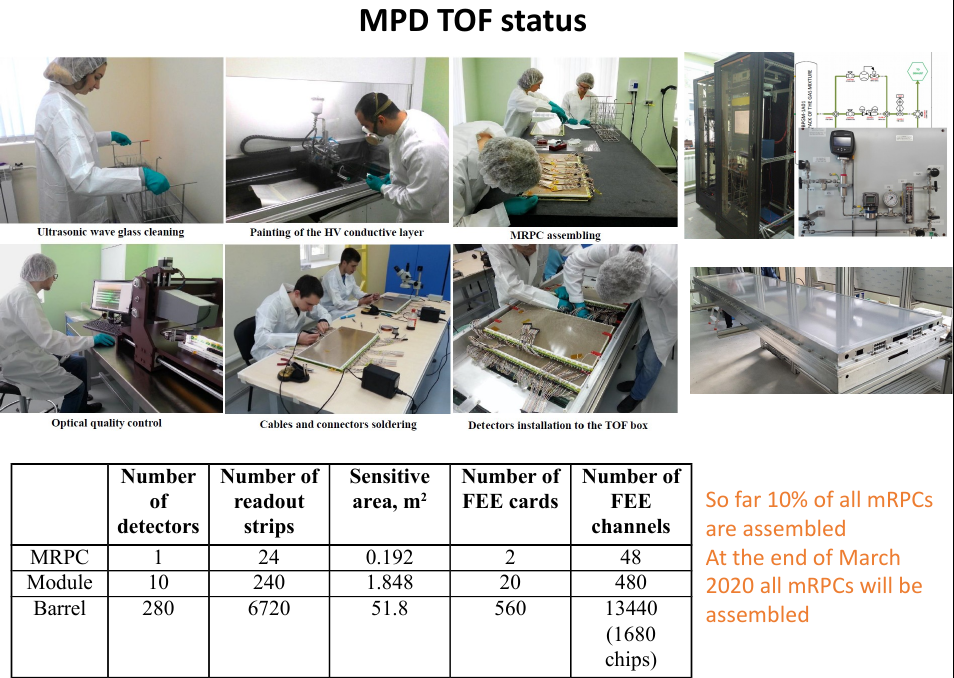
\includegraphics[width=1.\textwidth]{MPD_tofFabrication.png}
       \end{figure}
   \end{block}
     \column{.075\textwidth}
  \end{columns}
\end{frame}

\begin{frame}
  \frametitle {\bf \centering Assembling MPD ...}
   \vskip -0.05cm
  \begin{columns}[t]
     \column{.075\textwidth}
    \column{.90\textwidth}
   \begin{block}{}
       \begin{figure}[H]
         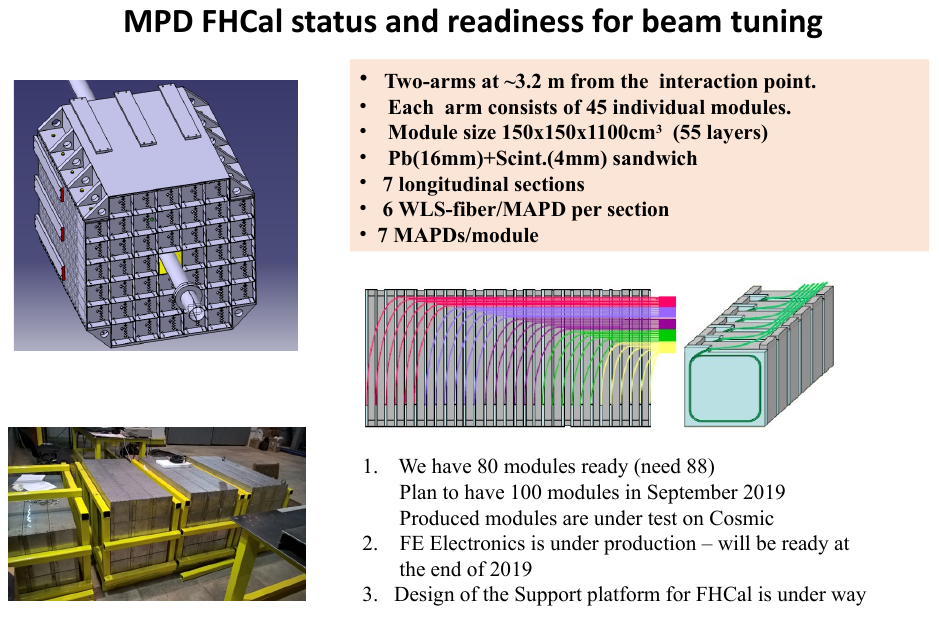
\includegraphics[width=1.\textwidth]{MPD_fhcalFabrication.png}
       \end{figure}
   \end{block}
     \column{.05\textwidth}
  \end{columns}
\end{frame}

\begin{frame}
  \frametitle {\bf \centering Assembling MPD ...}
   \vskip -0.75cm
  \begin{columns}[t]
     \column{.075\textwidth}
    \column{.90\textwidth}
   \begin{block}{}
       \begin{figure}[H]
         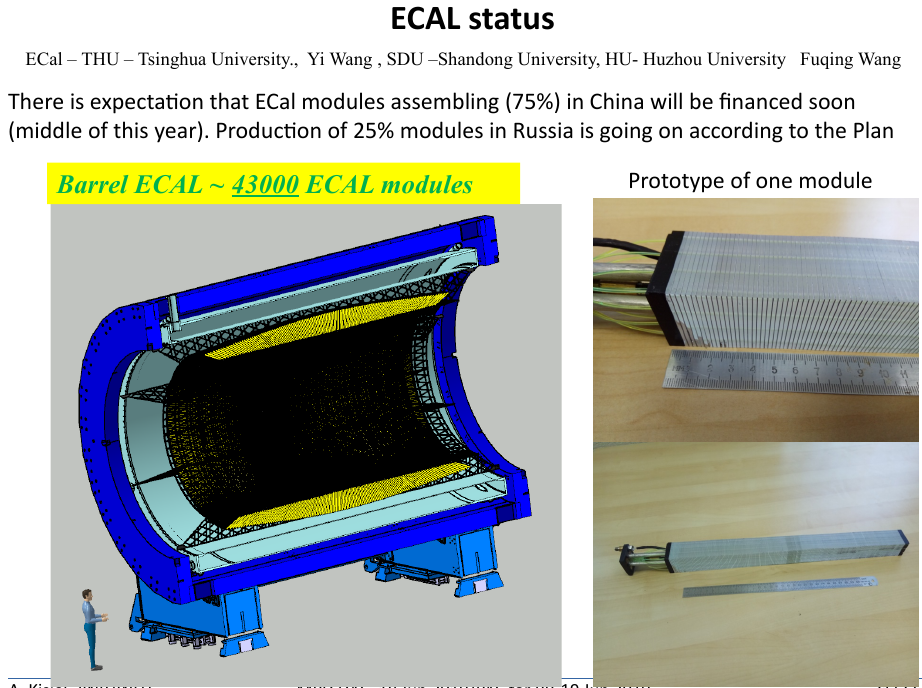
\includegraphics[width=1.\textwidth]{MPD_ecalFabrication.png}
       \end{figure}
   \end{block}
     \column{.05\textwidth}
  \end{columns}
\end{frame}

\begin{frame}
  \bf
  \frametitle{\bf \centering MPD physics cases}
             {\footnotesize
               \vskip -.7cm
               \begin{columns}[t]
                 \column{.49\textwidth}
                 \begin{block}{\bf \centering QCD phase diagram}
                   \begin{figure}[H]
                     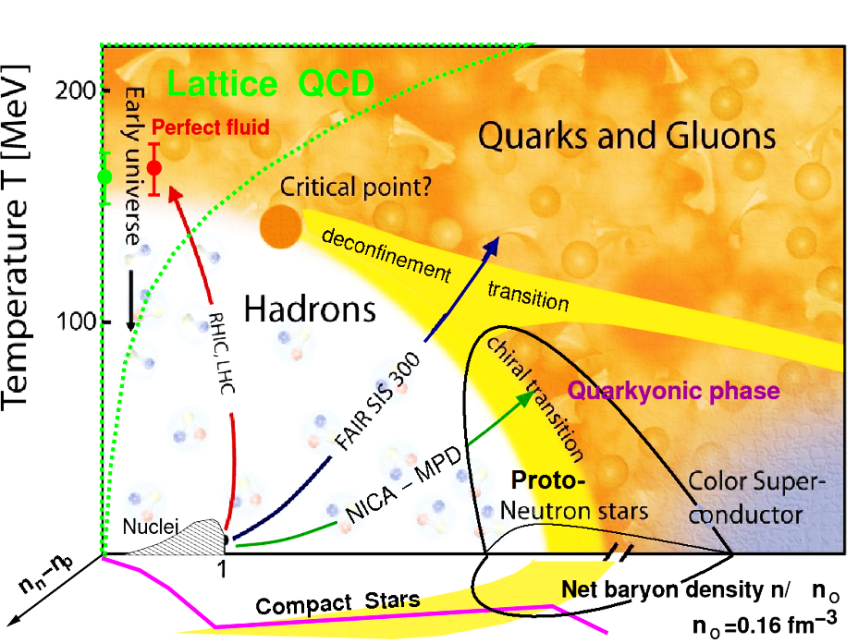
\includegraphics[width=1.\textwidth]{qcd_diagram.png} 
                   \end{figure}
                 \end{block}
                 \vskip -0.3cm
                 \begin{block}{\bf \centering Deconfinement (chiral) phase transition at high baryonic density}
                   % \vskip .25cm
                   \centering 
                       {\color{ForestGreen} enhanced strangeness production} \\
                       {\color{ForestGreen} Chiral Magnetic (vortical) effect, $\Lambda$-polarization}
                 \end{block}

                 \column{.49\textwidth}
                 \begin{block}{\bf \centering Bulk properties, EOS}
                   \centering
                       {\color{ForestGreen} particle yields \& spectra, ratios, femtoscopy, flow} \\
                       {\color {Red} measure: $\gamma$, $\pi$, $K$, $p$, $\Lambda$, $\Omega$, (anti)-particles, light nuclei}
                 \end{block}
                 \vskip -0.3cm
                 \begin{block}{\bf \centering In-Medium modification of hadron properties}
                   \centering 
                       {\color{ForestGreen} onset of low-mass dilepton enhancement} \\
                       {\color{Red} measure: $\rho$, $\omega$, $\phi$, $e^{+}e^{-}$}
                 \end{block}
                 \vskip -0.3cm
                 \begin{block}{\bf \centering QCD Critical Point}
                   \centering 
                       {\color{ForestGreen} event-by-event fluctuations and correlations}
                 \end{block}
                 \vskip -0.3cm
                 \begin{block}{\bf \centering Strangeness in nuclear matter}
                   \centering 
                       {\color{ForestGreen} hypernuclei}
                 \end{block}
               \end{columns}
             }
\end{frame}

\begin{frame}
  \frametitle{\bf \centering Multi-strangeness @ MPD}
  \bf
  \begin{columns}[t]
    \column{.33\textwidth}
    \vskip -.75cm
    \begin{block}{\bf \centering {\scriptsize Hyperon yields for 1 week of running (Stage 1)}}
      % \begin{table}[H]
      % \vskip -1cm
      % \caption{Hyperon yields for 1 week of running (Stage 1)}
      % \vskip -0.65cm
      \resizebox{\columnwidth}{!}{%
        %\captionof{table}{Your caption here}
        \begin{tabular}{| l | l |}
          \hline			
          Particle & Yield \\
          \hline
          $\Lambda^{0}$ & $3 \cdot 10^{7}$ \\
          \hline
          $\overline{\Lambda}^{0}$ & $3.5 \cdot 10^{5}$ \\
          \hline
          $\Xi^{-}$ & $1.5 \cdot 10^{5}$ \\
          \hline
          $\overline{\Xi}^{+}$ & $8.0 \cdot 10^{3}$ \\
          \hline
          $\Omega^{-}$ & $7 \cdot 10^{3}$ \\
          \hline
          $\overline{\Omega}^{+}$ & $1.5 \cdot 10^{3}$ \\
          \hline
        \end{tabular}     
      }
      % \end{table}
    \end{block}
    \vskip -.25cm
    \begin{block}{}
      \begin{figure}[H]
        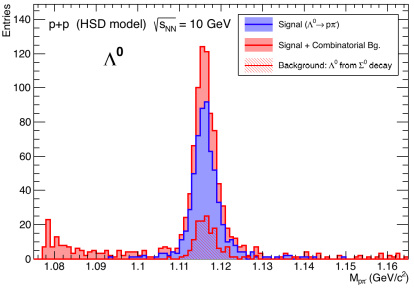
\includegraphics[width=1.\textwidth]{lambda_recoMPD.png}
      \end{figure} 
    \end{block}     

    \column{.3\textwidth}
    \vskip -.75cm
    \begin{block}{\bf \centering Decay topology}
      \begin{figure}[H]
        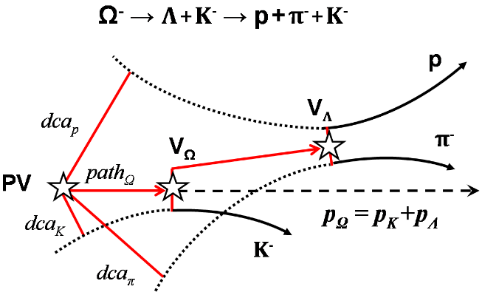
\includegraphics[width=1.\textwidth]{secDecay_topology.png} 
      \end{figure} 
    \end{block}
    \vskip -.40cm
    
    \begin{block}{}
      \vskip -.17cm
      \begin{figure}[H]
        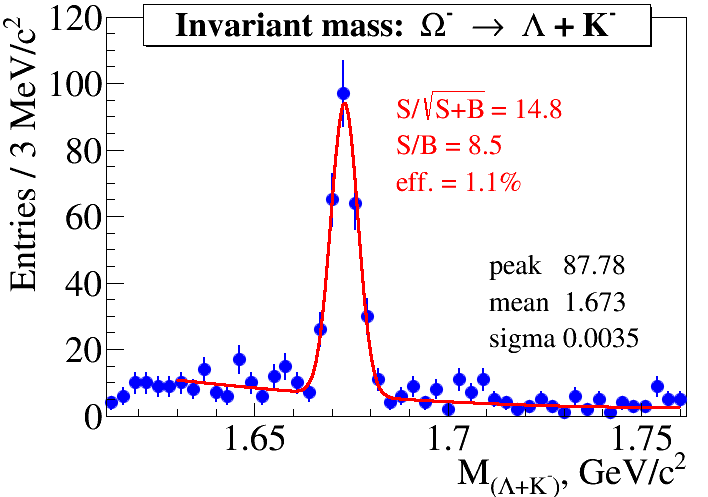
\includegraphics[width=1.\textwidth]{omega_minus.png} 
      \end{figure}
      \vskip -.9cm
      \begin{figure}[H]
        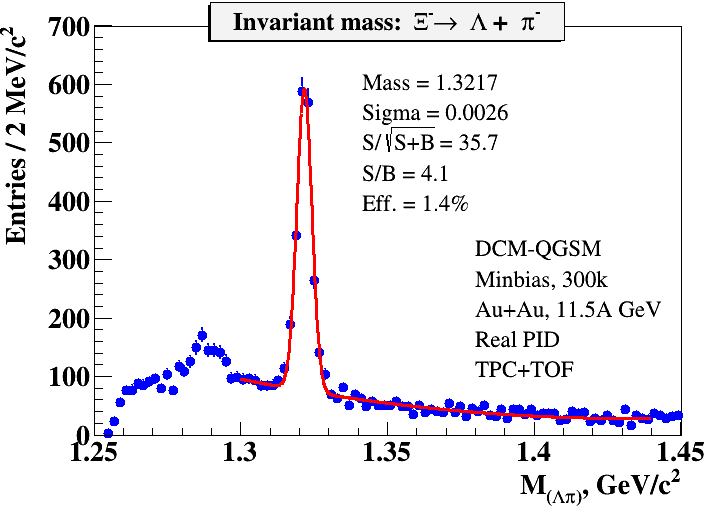
\includegraphics[width=1.\textwidth]{ksi_minus.png} 
      \end{figure}     
    \end{block}
    
    
    \column{.33\textwidth}
    \vskip -.75cm
           {\tiny
             \begin{block}{\bf \centering Data \& Analysis}
               \begin{itemize}
               \item $5 \cdot 10^{5}$ events, AuAu @ $\sqrt{s_{NN}} = 9$ GeV
               \item $\Lambda$-candidates are in inv. mass window $\pm 3\sigma$
               \item Topological cuts are optimized to improve significance 
               \end{itemize}
               \vskip -.65cm
               \begin{figure}[H]
                 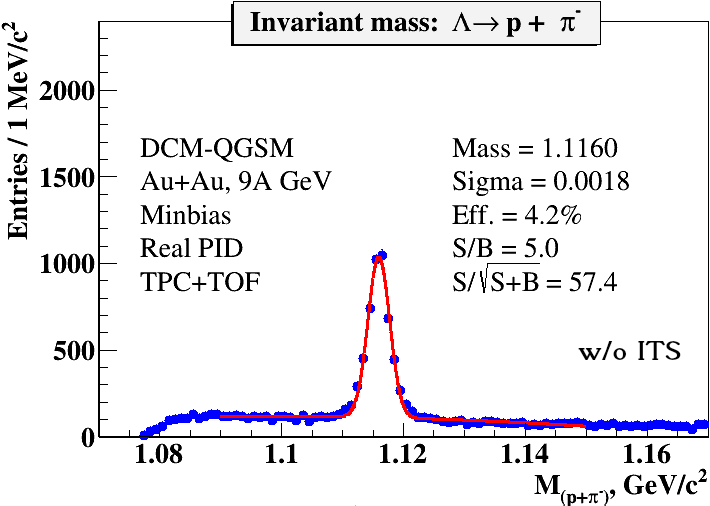
\includegraphics[width=1.\textwidth]{lambda_noITS.png} 
               \end{figure}
               \vskip -.85cm
               \begin{figure}[H]
                 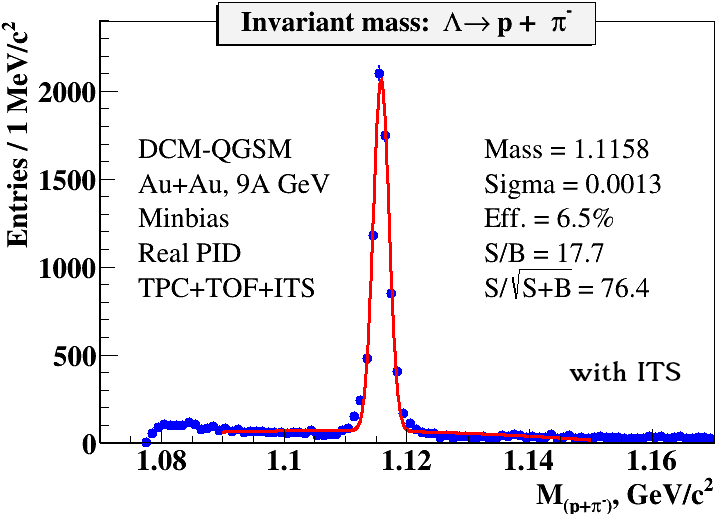
\includegraphics[width=1.\textwidth]{lambda_wITS.png}
               \end{figure}
             \end{block}
           }
  \end{columns}
  \note{\note{Production of strange particles in A+A collisions is of particular interest because their
                 enhanced yields (relative to pp reactions) have been predicted as the signal of the deconfinement phase
                 transition. Such enhancement, indeed, was observed at SPS energies and then confirmed at the RHIC.
                 However, the data on strangeness production, especially at threshold, at energy region of the maximum baryonic
                 density are not complete or even missing}}
\end{frame}

\begin{frame}
  \bf 
  \frametitle{\bf \centering Hypernuclei @ MPD}
  \begin{columns}[t]
    \column{.31\textwidth}
    \vskip -.77cm
    \begin{block}{\bf \centering Particle Identification}
      \begin{figure}[H]
        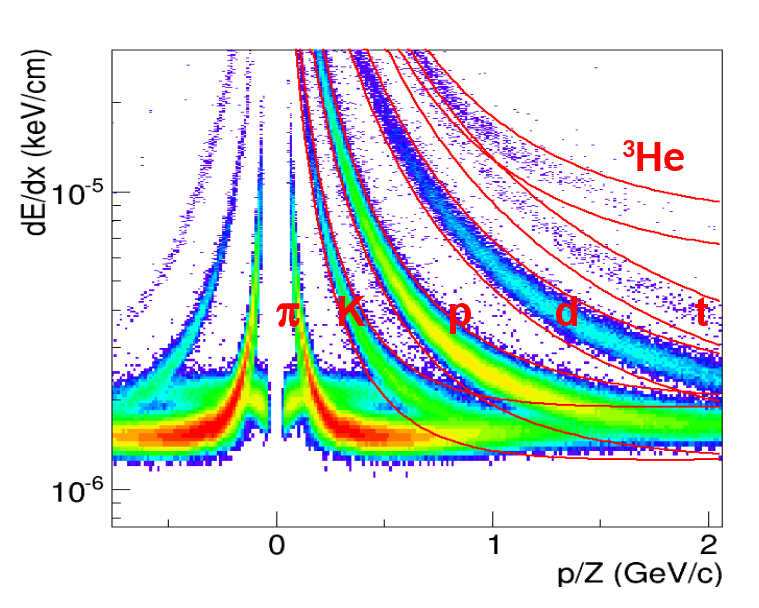
\includegraphics[width=1.\textwidth]{pid_dEdX.png} 
      \end{figure}
      \vskip -.55cm
      \begin{figure}[H]
        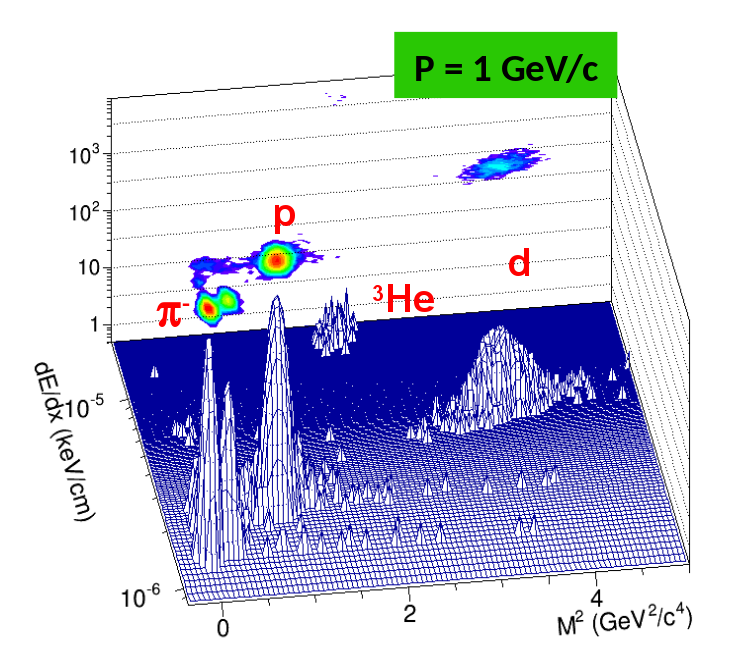
\includegraphics[width=1.\textwidth]{pid_dEdX_ToF.png} 
      \end{figure}     
    \end{block}

    \column{.31\textwidth}
    \vskip -.8cm
    \begin{block}{\bf \centering {\scriptsize Decay topology}}
      \begin{figure}[H]
        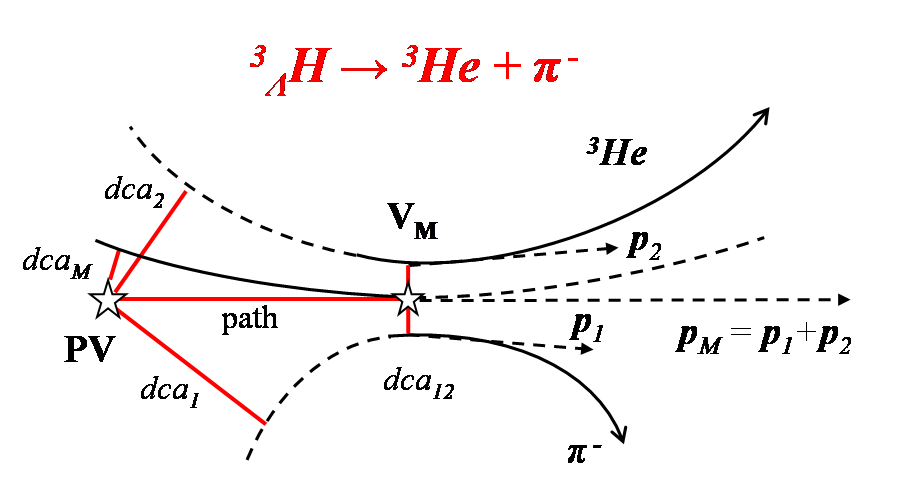
\includegraphics[width=1.\textwidth]{He3pion_invMass_topology.png} 
      \end{figure}
    \end{block}
    \vskip -.4cm
           {\tiny
             \begin{block}{\bf \centering {\scriptsize Data \& Analysis}}
               \begin{itemize}
               \item Particles are selected within $\pm 3\sigma$-cuts in $dE/dx$ or $dE/dx - M^{2}$
               \item $V_{0}$ finding is done with quality cuts for max. significance 
               \end{itemize}
             \end{block}
           }
           \vskip -.4cm
           \begin{block}{\bf \centering {\scriptsize ``Strong'' cuts}}
             \begin{figure}[H]
               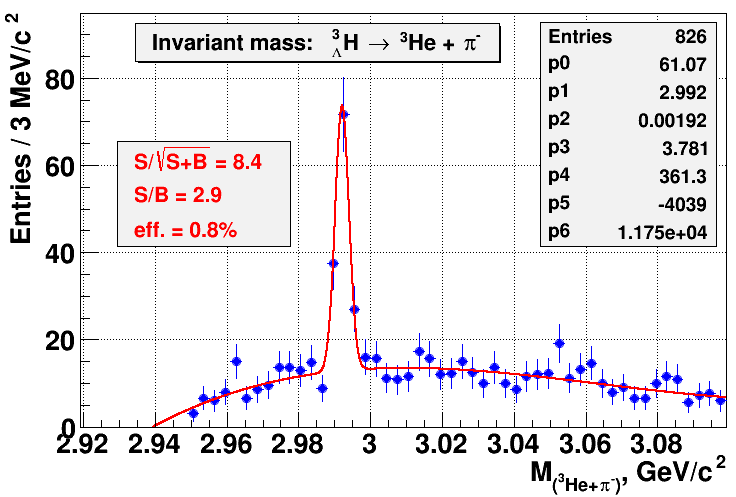
\includegraphics[width=1.\textwidth]{He3pion_invMass_maxCuts.png} 
             \end{figure}
             
           \end{block}
           
           \column{.31\textwidth}
           \vskip -.757cm
           \begin{block}{\bf \centering {\scriptsize ``Soft'' cuts}}
             \begin{figure}[H]
               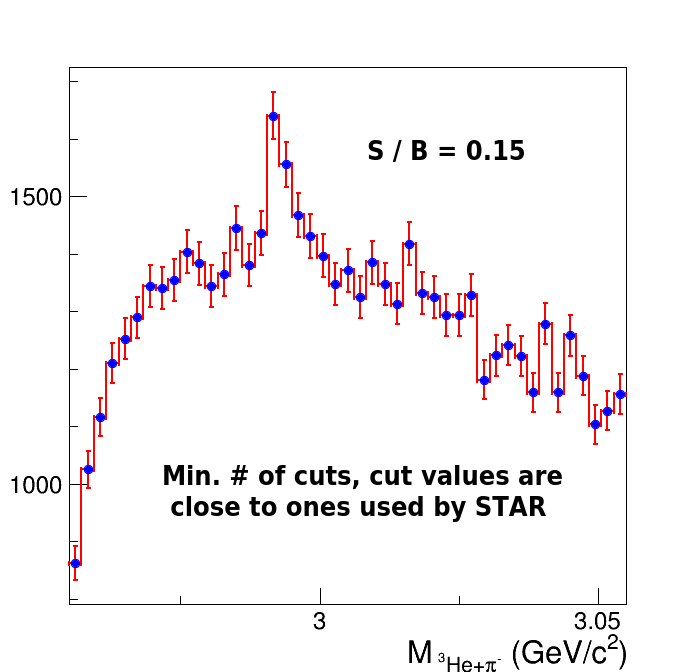
\includegraphics[width=1.\textwidth]{He3pion_invMass_minCuts.png} 
             \end{figure}
           \end{block}
           \vskip -.35cm
           \begin{block}{\bf \centering {\scriptsize STAR preliminary}}
             \begin{figure}[H]
               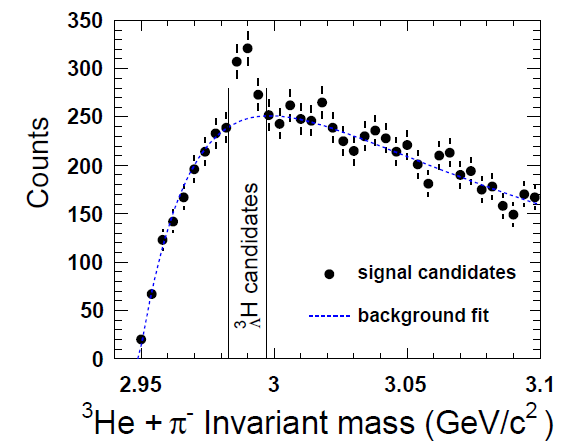
\includegraphics[width=1.\textwidth]{He3pion_invMass_STAR.png} 
             \end{figure}
           \end{block}
  \end{columns}
  \note{
    Hypernuclei provide unique opportunity to study hyperon-nucleus interactions in a many-body environment.
    Details of the strange sector in the nuclear matter equation-of-state (EOS) are of great importance for astrophysics
    and should help understanding the mechanism of creation and evolution of super-dense stellar objects - neutron stars.
    Results of model calculations indicate, the yields of hypernulei in central heavy ion collisions are enhanced within
    the NICA energy range, this gives good perspectives for such kind of studies at NICA.
    Hypernuclei could be reliably reconstructed and detected using PID based
    on the measurements of ToF and energy losses due to ionization in TPC
    An analysis of the hypernuclei reconstruction has been performed with
    $5 \cdot 10^{5}$ central Au+Au events, which corresponds to about 30 minutes of data taking time at NICA.
    The obtained invariant mass spectra for reconstruction of two modes of simulated hypertriton decays are presented.}
\end{frame}

\begin{frame}
  \frametitle{\bf \centering Dileptons @ MPD}
  \bf
  \vskip -.75cm
  \begin{columns}[t]
    \column{.605\textwidth}
    %\vskip -.65cm
    \begin{block}{\bf \centering {\scriptsize Invariant mass of dileptons (background subtracted): red - MC, blue - reco}}
      \begin{figure}[H]
        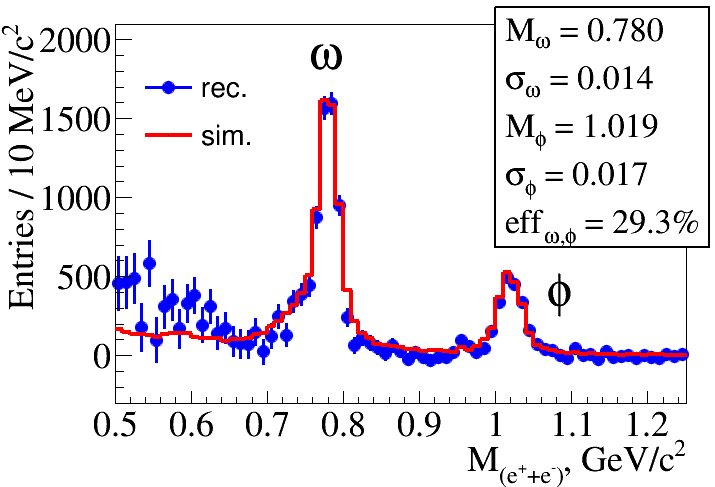
\includegraphics[width=1.\textwidth]{dileptons_invmass.png} 
      \end{figure}
    \end{block}
    \vskip -.3cm
    \begin{block}{\bf \centering {\scriptsize Yield, decay modes ... for dileptons}}
      % \begin{table}[H]
      % \vskip -1cm
      % \caption{Hyperon yields for 1 week of running (Stage 1)}
      % \vskip -0.65cm
      \resizebox{\columnwidth}{!}{%
        %\captionof{table}{Your caption here}
        \begin{tabular}{| c | c | c | c | c | c | c |}
          \hline         
	  \multirow{2}{*}{Particle} & \multicolumn{2}{|c|}{Yield} & \multirow{2}{*}{Decay mode} & \multirow{2}{*}{BR} & \multirow{2}{*}{Eff. [\%]} &
          \multirow{2}{*}{Yield [per 1 week]} \\ 
          %\hline
          \cline{2-3}
          & $4\pi$ & y = 0 & & & & \\
          \hline
          $\rho$ & 31 & 17 & $e^{+}e^{-}$ & $4.7 \cdot 10^{-5}$ & {\color{red} 35} & $7.3 \cdot 10^{4}$\\
          \hline
          $\omega$ & 20 & 11 & $e^{+}e^{-}$ & $7.1 \cdot 10^{-5}$ & {\color{red} 35} & $7.2 \cdot 10^{4}$ \\
          \hline
          $\phi$ & 2.6 & 1.2 & $e^{+}e^{-}$ & $3 \cdot 10^{-4}$ & {\color{red} 35} & $1.7 \cdot 10^{4}$\\
          \hline
        \end{tabular}     
      }
    \end{block}
    \vskip -.3cm
     \begin{block}{\bf \centering {\tiny Estimate of  dilepton yield in central Au+Au at $M_{inv}$ = $2 - 2.5 GeV/c^{2}$}}
      \resizebox{\columnwidth}{!}{%
        \begin{tabular}{| c | c |}
          \hline
          $\sqrt{s_{NN}}~~[GeV]$ & $N_{pairs}$ [per 10 days] \\
          \hline
          6.3 & 54 \\
          \hline
          8.0 & 410 \\
          \hline
        \end{tabular}

      }
    \end{block}
    \column{.375\textwidth}
    %\vskip -.65cm
    \begin{block}{\bf \centering PID}
       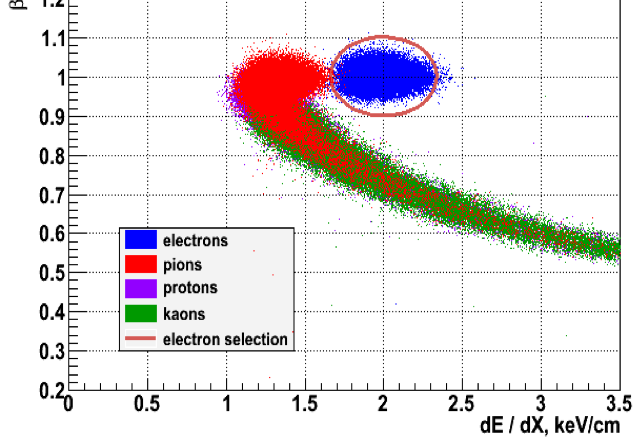
\includegraphics[width=1.\textwidth]{dileptons_PID.png}
    \end{block}
    \vskip -.3cm
    \begin{block}{\bf \centering {\scriptsize MPD \\ \vskip -0.09cm $0.2 < M_{(e^{+}e^{-})} < 1.1 GeV/c^{2}$}}
      \begin{figure}[H]
        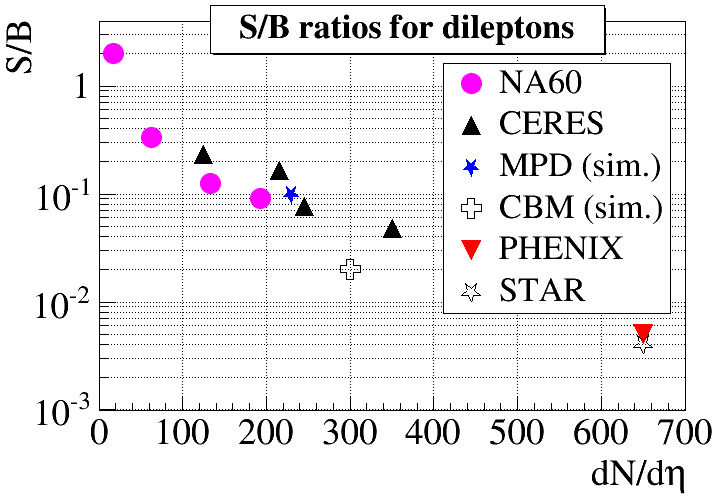
\includegraphics[width=1.\textwidth]{StoB_dileptons.png} 
      \end{figure}
    \end{block}
  \end{columns}
  \note{If the deconfinement phase transition in dense hadronic matter is accomplished by partial restoration of the chiral
    symmetry, the vector meson spectral functions can be modified. Electron-positron pairs (dileptons) from vector meson decays
    are in this case the best candidates to study such in-medium modifications since they interact only weakly and escape easily
    having no subsequent strong interactions in the nuclear medium.
    The reliable electron identification using the combined information from the TOF and TPC detectors.
    Additional information on the energy deposit from the ECAL calorimeter allows reducing the hadron
    contamination in the electron sample down to the level of $10^{-5}$.
    That could provide the reliable vector meson reconstruction though their dilepton decays in heavy-ion collisions at MPD
  }
\end{frame}

\begin{frame}
  \bf
  \frametitle{\bf \centering Flow @ MPD}
  \vskip -.75cm
  \begin{columns}[t]
    \column{.49\textwidth}
    \begin{block}{\bf \centering Direct flow}
      \vskip -.1cm
      \begin{figure}[H]
        \includegraphics[width=1.\linewidth]{dv1_dy_v1.pdf}
      \end{figure}
      \vskip -.7cm
             {\scriptsize {\color{Red} Slope of $v_{1}$ changes sign in the NICA energy range}}
    \end{block}
    
    \column{.49\textwidth}
    \begin{block}{\bf \centering Elliptic flow}
      \vskip -.1cm
      \begin{figure}[H]
        \includegraphics[width=1.\linewidth]{v2edep.pdf}
      \end{figure}
      \vskip -.65cm
             {\scriptsize {\color{Red} $v_{2}$ becomes very close to zero in the NICA energy range}}
    \end{block}
    \vskip -.3cm
           {\tiny
             \vskip -.05cm
             \begin{block}{}
               \vskip -.1cm
               \begin{itemize}
               \item Large uncertainties in existing experimental data in the NICA energy range
               \item Non-monotonic $|dv_{1}/dy|_{y=0}$ behavior could be a signature of phase transition
               \item More differential (centrality classes) measurements required 
               \end{itemize}
             \end{block}
           }
  \end{columns} 
\end{frame}
  
\begin{frame}
  \bf
  \frametitle{\bf \centering Femtoscopy @ MPD with vHLLE+UrQMD}
  \vskip -.75cm
  \begin{columns}[t]
    \column{.30\textwidth}
    \begin{block}{\bf \centering {\tiny Thermodynamic pressure as a function of energy density}}          
      \vskip -.1cm
      \begin{figure}[H]
        % \caption{Thermodynamic pressure as a function of energy density, 
        %evaluated at zero baryon density from the equations of state used in the hydrodynamic stage: 
        %chiral model EoS with crossover transition (XPT) and bag model EoS with first order phase transition (1PT).}
        \includegraphics[width=1.01\linewidth]{eos.eps}
      \end{figure}
    \end{block}
    
    \column{.32\textwidth}
    \begin{block}{\bf \centering {\tiny Parameters $\tau_0$, $R_\perp$, $R_\eta$ and $\eta/s$ adjusted using basic
          observables in the RHIC BES region.}}        
      %\vskip -.3cm
      \resizebox{\columnwidth}{!}{%       
        \begin{tabular}{|l|l|l|l|l|}
          \hline
          $\sqrt{s_{\rm NN}}$~[GeV] & $\tau_0$~[fm/c] & $R_\perp$~[fm] & $R_\eta$~[fm] & $\eta/s$ \\ \hline
          7.7          &      3.2        &     1.4        &     0.5    &    0.2   \\ \hline
          8.8 (SPS)    &      2.83       &     1.4        &     0.5    &    0.2   \\ \hline
          11.5         &      2.1        &     1.4        &     0.5    &    0.2   \\ \hline
          17.3 (SPS)   &      1.42       &     1.4        &     0.5    &    0.15  \\ \hline
          19.6         &      1.22       &     1.4        &     0.5    &    0.15  \\ \hline
          27           &      1.0        &     1.2        &     0.5    &    0.12  \\ \hline
          39           &      0.9        &     1.0        &     0.7    &    0.08  \\ \hline
          62.4         &      0.7        &     1.0        &     0.7    &    0.08  \\ \hline
          200          &      0.4        &     1.0        &     1.0    &    0.08  \\ \hline
        \end{tabular}
      }
    \end{block}
    
    \column{.32\textwidth}  
    \begin{block}{\bf \centering {\tiny Pion emission times at the last interaction}}
      \begin{figure}[H]
        \includegraphics[width=1.\linewidth]{fig1a_poster.eps}
      \end{figure}
      \vskip -.6cm
             {\bf \tiny {\color{Red} Phys. Rev. C 96, 024911 (2017)}}
    \end{block}
  \end{columns}
  \begin{columns}[c]
    \column{.49\textwidth}
    \vskip -.3cm
    \begin{block}{\bf \centering {\tiny Comparison of extracted radii with the STAR data}}
      % \vskip .3cm
      \begin{figure}[H]
        \includegraphics[width=1.0\linewidth]{fig4_poster.eps}
      \end{figure}
     % \vskip -.75cm
      %      \begin{figure}[H]
      %       \includegraphics[width=1.\linewidth]{fig5.pdf}
      %\caption{Ratio of the ``out'' and ``side'' radii (top) and difference of the radii squared (bottom) 
      %as a function of $\sqrt{s_{NN}}$ derived from the STAR data ($0.15 < k_{T} < 0.25$ GeV/c, 0-5\% centrality) 
      %and compared with the model calculations using the two EoS's.}
      %    \end{figure}
    \end{block}
    \column{.49\textwidth}
    \vskip -.3cm
    \begin{block}{}
      {\scriptsize
        \begin{itemize}
        \item {\color{Red} EoS with a crossover in the fluid phase} results in a quite reasonable reproduction of 3D pion femtoscopic radii measured by the STAR collaboration (empty squares).
        \item {\color{ForestGreen} EoS with a first-order phase transition} leads to fact that the ``out'' and ``long'' Gaussian femtoscopic radii are systematically larger
          if comparing with the {\color{Red} crossover EoS}; the ``side'' radii coincide for both types of EoS.
          % \item  No readjustment for the 1PT EoS poses an open question whether the differences in femtoscopic radii between the two EoS's will be even smaller if the readjustment is made for each EoS scenario individually.  
        \end{itemize}
      }
    \end{block}
  \end{columns}
\end{frame}


\begin{frame}
  \bf
  \frametitle{\bf \centering Observables @ MPD with THESEUS}
  \vskip -.8cm
  \begin{columns}[t]
    \column{.23\textwidth}
    \begin{block}{\bf \centering {\footnotesize $|dv_{1} / dy|_{y=0}$ \\protons}}
      \begin{figure}[H]
        \includegraphics[width=1.0\linewidth]{proton_fig5_THESEUS_zeroLine_corrected.pdf} 
      \end{figure}
    \end{block}
    \column{.23\textwidth}
    \begin{block}{\bf \centering {\footnotesize $|dv_{1} / dy|_{y=0}$ \\ pions}}
      \begin{figure}[H]
        \includegraphics[width=1.0\linewidth]{pion_fig6_THESEUS_zeroLine_corrected.pdf}
      \end{figure}
    \end{block}
    \column{.23\textwidth}
    \begin{block}{\bf \centering {\scriptsize Curvature of net-proton rapidity distribution}}
      \vskip -.2cm
      \begin{figure}[H]
        \includegraphics[width=1.0\linewidth]{graphs_Cy_central.pdf}
      \end{figure}
    \end{block}
    \column{.23\textwidth}
    \begin{block}{\bf \centering {\footnotesize The "horn'' effect?}}
      \begin{figure}[H]
        \includegraphics[width=1.0\linewidth]{fig9_THESEUS_thickErrBars.pdf}
      \end{figure}
    \end{block}
  \end{columns}
   \vskip -.4cm
  \begin{columns}[t]   
    \column{.49\textwidth}
    {\tiny
    \begin{block}{}
      \begin{itemize}
      \item Hadronic cascade has a small effect on $dv_{1} / dy$ for protons
      \item Hadronic cascade changes flow to antiflow for pions at low energies.
        The effect becomes weaker with the collision energy rise. 
      \end{itemize}
    \end{block}
    }
    \column{.23\textwidth}
    {\tiny
      \begin{block}{}
       \vskip -.1cm
      \begin{itemize}
      \item The ``wiggle'' as a feature for the EoS with a 1-st order phase transition is robust against hadronic FSI.
      \end{itemize}
    \end{block}
    }
   % }
    \column{.23\textwidth}
    {\tiny
    \begin{block}{}
      \begin{itemize}
      \item Turning the hadronic cascade on does not influence the kaon to pion ratio.
      %\item As the 3FH-model itself, also THESEUS in its present version is not yet capable of describing the ”horn” effect.
      \end{itemize}
    \end{block}
    }
  \end{columns}
  \note{{\tiny Next we test whether more subtle features of particle distributions are preserved by the particlization procedure
    and how they are affected by the hadronic cascade.
    First we calculate the directed flow coefficient v1 for pions and protons as a function of rapidity using the
    reaction plane method. On the slide we present the distributions in a condensed form using the slope of the directed flow
    at midrapidity dv1/dy calculated in the interval $|\Delta y|$ < 0.5 around midrapidity.
    Dashed lines show the results from THESEUS without hadronic cascade, where we quantitatively reproduce the results from
    basic 3FH model for the EoS with a first-order phase transition denoted as ``2-phase EoS''.
    Turning the UrQMD hadronic cascade on for the final state we observe that the cascade has only
    a small effect on the excitation function of the proton dv1/dy.
    However, for the pions the hadronic cascade changes flow to antiflow at low energies.
    This behaviour can be understood as follows. If there is only hydrodynamics, the pions are emitted along the fluid flow,
    while when there is rescattering they are blocked by the baryonic matter in the projectile and target region,
    therefore the antiflow appears. The effect of the pion shadowing becomes weaker with the collision energy rise,
    because the midrapidity region becomes less baryon abundant.} }
\end{frame}

\begin{frame}
  \bf
  \begin{block}{}
    \begin{center}
      {\Huge Experiments in fixed-target mode}
    \end{center}
  \end{block}
\end{frame}

\begin{frame}
  \frametitle{\bf \centering BM@N experiment}
  \bf
       \vskip -.8cm
       \begin{columns}[t]
         \column{.69\textwidth}
         \begin{block}{\bf \centering Full setup, layout}
           \begin{figure}[H]
             \includegraphics[width=1.\linewidth]{bmn_fullConfig.png}
           \end{figure}
         \end{block}

         \column{.29\textwidth}
         {\tiny
           \begin{block}{}
             \begin{itemize}
             \item Central tracker (Silicon tracker + GEM) inside analyzing magnet to reconstruct
               AA-interactions
             \item Outer tracker (CPC, DCH) behind magnet to link tracks from central tracker to ToF detectors
             \item TOF1 \& TOF2 system based on mRPC and T0 detectors to identify hadrons and light nuclei
             \item Detectors to form T0 and beam monitors
             \item ZDC calorimeter to measure centrality of AA-collisions
             \item Electromagnetic calorimeter for $\gamma$, $e^{+}$, $e^{-}$
             \end{itemize}
           \end{block}
         }
       \end{columns}
       \vskip -.2cm
       {\footnotesize
         \begin{block}{\bf \centering {\scriptsize  BM@N advantages:}}
           \vskip -.1cm
         \begin{itemize}
         \item \centering large aperture analyzing magnet
         \item sub-detector systems are resistant to high multiplicities of charged particles
         \item PID: "near to magnet" (TOF1), "far from magnet" (TOF2)
         \end{itemize}
       \end{block}
       }
\end{frame}

\begin{frame}
  \bf
  \frametitle{\bf \centering {\footnotesize Exploring high density baryonic matter with Nuclotron}}
  \vskip -.75cm
  \begin{columns}[t]
    \column{.51\textwidth}
    \begin{block}{}
      \includegraphics[width=1.\linewidth]{bar_densities.png}
    \end{block}
    \column{.47\textwidth}
       \begin{block}{}
         \includegraphics[width=1.\linewidth]{barDensDomination.png}
       \end{block}
\end{columns}
  \begin{block}{}
    \begin{center}
  Nuclotron is well suited to study high density (dominantly baryonic) matter since at that energies
  baryon-dominated system exists comparatively long lifetime
    \end{center}
  \end{block}
\end{frame}

\begin{frame}
  \bf
  \frametitle{Physics possibilities at the Nuclotron}
  % {\small
  \vskip -.75cm
               \begin{columns}[t]
                 \column{.49\textwidth} 
                 \begin{block}{\bf \centering $A+A$ collisions:}
                   \begin{itemize}
                   \item strangeness at threshold
                   \item Need more precise data for strange mesons, hyperons and hypernuclei, multi-variable distributions, unexplored energy range
                   \end{itemize}
                 \end{block}
                 \begin{block}{\bf \centering $p+p$, $p+n$, $p+A$ collisions:}
                   \begin{itemize}
                   \item Hadron production in elementary reactions and ``cold'' nuclear matter as a ``reference'' to determine exactly nuclear effects 
                   \end{itemize}
                 \end{block}
                 
                 \column{.44\textwidth} 
                 \begin{block}{\centering \bf {\color{yellow}{AGS}} {\color{red}{NA49}} {\color{ForestGreen}{BRAHMS}}}
                   %  \includegraphics[width=.4\linewidth]{strangeness_prod.png}
                   \includegraphics[width=1.\linewidth]{strangeness_prod.png}
                 \end{block}
                 %\begin{block}{}
                  % \includegraphics[width=1.\linewidth]{horn_NA49.png}
                 %\end{block}
               \end{columns}
               %  }
               \note{Production of strange particles in A+A collisions is of particular interest because their
                 enhanced yields (relative to pp reactions) have been predicted as the signal of the deconfinement phase
                 transition. Such enhancement, indeed, was observed at SPS energies and then confirmed at the RHIC.
                 However, the data on strangeness production, especially at threshold, at energy region of the maximum baryonic
                 density are not complete or even missing}
\end{frame}

\begin{frame}
  \bf
  \frametitle{Heavy ions $A+A$: Hypernuclei production}
  \vskip -.75cm
  \begin{columns}[t]
    \column{.49\textwidth}
    \begin{block}{{\tiny \bf \centering A. Andronic et al., Phys. Lett. B697 (2011) 203}}
      \includegraphics[width=1.\linewidth]{hypernucl_prod.png}
    \end{block}
    \vskip -.2cm
    \begin{block}{}
    \centering 
        {\color{ForestGreen} BM@N energy range} is {\color{red} suited} for the search of (double) hypernuclei
  \end{block}
    \column{.49\textwidth}
    \begin{block}{}
      \includegraphics[width=1.\linewidth]{dNdY_asAdep.png}
    \end{block}
    \vskip -.3cm
    {\scriptsize
      \begin{block}{}
        \vskip -.1cm
       \begin{itemize}
      \item {\color{red} In heavy-ion collisions:} production of hypernuclei through coalescence of $\Lambda$
        with light fragments enhanced at high baryon densities
      \item {\color{red} Maximal yield} predicted for $\sqrt{s_{NN}}$ = 4 - 5~AGeV (stat. model)
        %(interplay of $\Lambda$ and light nuclei excitation function)
     \end{itemize}
     \end{block}
     }
  \end{columns}
  \note{Hypernuclei provide unique opportunity to study hyperon-nucleus interactions in a many-body environment.
    Details of the strange sector in the nuclear matter equation-of-state (EOS) are of great importance for astrophysics
    and should help understanding the mechanism of creation and evolution of super-dense stellar objects - neutron stars.
    Results of model calculations indicate, the yields of hypernulei in central heavy ion collisions are enhanced within
    the NICA energy range, this gives good perspectives for such kind of studies at NICA.}
\end{frame}

\begin{frame}
  \bf
  \frametitle{\bf \centering BM@N feasibility study}
  \vskip -.3cm
   \begin{block}{}
      Simulation: UrQMD \& DCM-QGSM, Au+Au,  T = 4.5 AGeV
   \end{block}
   \vskip -.5cm
  \begin{columns}[t]   
    \column{.49\textwidth}
    \begin{block}{}
      \begin{center}
      900k central events, \\
      7.5M  $\Xi^{-}$ in 1 month \\
      20 kHz trigger
      \end{center}
    \end{block}
    \vskip -.2cm
    \begin{block}{}
       \includegraphics[width=1.\linewidth]{BMN_ksi.png}
    \end{block}
    \column{.49\textwidth}
    \begin{block}{}
      \begin{center}
      2.6M central events, \\
      8.5M  \ce{^{3}_{$\Lambda$}H} in 1 month \\
      20 kHz trigger
      \end{center}
    \end{block}
    \vskip -.2cm
     \begin{block}{}
       \includegraphics[width=1.\linewidth]{BMN_hyperTrit.png}
    \end{block}
  \end{columns}
  \begin{block}{}
    \begin{center}
      \bf The feasibility study indicates reliable reconstruction of cascades and hypernuclei of order of 10 millions per month
    \end{center}
    \end{block}
  \note{}
\end{frame}

\begin{frame}
  \bf
  \frametitle{\bf \centering BM@N, carbon run}
  \vskip -.1cm
 % \begin{block}{\bf \centering Setup:}
    \includegraphics[width=1.\linewidth]{bmn_winter2016_config_common_view_labels.png}
 % \end{block}
  \vskip -.7cm
  {\tiny
  \begin{columns}[t]
    \column{.23\textwidth}
    \begin{block}{\bf \centering {\scriptsize Input beams:}}
      Deuteron beam (d), $T= 4.0, 4.6$ AGeV \\
      Carbon beam (C), $T = 3.5, 4.0,  4.5$ AGeV
    \end{block}
    \column{.33\textwidth}
    \begin{block}{\bf \centering {\scriptsize Aims:}}
      \begin{itemize}
      \item Focus on tests and commissioning  of central tracker inside analyzing magnet $\rightarrow$ GEM detectors and forward Si detector for tracking
      \item Test / calibrate ToF, trigger detectors, calorimeters
      \end{itemize}
    \end{block} 

    \column{.33\textwidth}
    \begin{block}{\bf \centering {\scriptsize Program:}}
      \begin{itemize}
      \item Trace beam through detectors, align detectors, measure beam momentum in mag. field of 0.3 - 0.85 T
      \item Measure inelastic reactions d (C) + target $\rightarrow$ X  with deuteron and carbon beam energies of 3.5 - 4.6 GeV/n on targets $CH_{2}$, C, Al, Cu, Pb
      \end{itemize}
    \end{block}
  \end{columns}
  }
\end{frame}

\begin{frame}
  \vskip -.8cm
  \frametitle{\bf \centering  {$\Lambda^{0}$ in deutron and carbon runs}}
  \begin{columns}[t]
    \column{.35\textwidth}
    {\footnotesize 
     \begin{block}{}
       \bf
       \begin{center}
       d (C) + target $\rightarrow$ X \\
       $\Lambda^{0}$-signal width $\sim$ 2.5-3 MeV
       \end{center}
     \end{block}
    % \vskip -.3cm
    % \begin{block}{}
    %   \begin{center}
    %     {\color{red} \bf No detailed PID used}
    %   \end{center}
    % \end{block}
     }
    % \vskip -.3cm
     \begin{block}{\bf \centering {\footnotesize Deuteron run}}
       \begin{figure}[H]
         \includegraphics[width=1.\linewidth]{lambda_run5.png} 
       \end{figure}
     \end{block}
    \column{.60\textwidth}
    \begin{block}{\bf \centering {\footnotesize Carbon run, T = 4 AGeV}}  
      \begin{minipage}{.49\linewidth}
        \includegraphics[width=1.\linewidth]{lambda_all.png} \\ 
        \includegraphics[width=1.\linewidth]{lambda_Cu.png}
      \end{minipage}
      \begin{minipage}{.49\linewidth}
        \includegraphics[width=1.\linewidth]{lambda_C.png} \\
        \includegraphics[width=1.\linewidth]{lambda_Al.png}
      \end{minipage}
    \end{block}
  \end{columns}
  \vskip -.3cm
  \begin{columns}[t]
    \column{.29\textwidth}
    \begin{block}{}
      \vskip -.1cm
      \bf
      {\footnotesize {\color{blue} PEPAN Lett., v.15, p.136, 2018(2):} {\color{red} First results from BM@N technical run with deuteron beam}}
    \end{block}
    \column{.68\textwidth}
   \begin{block}{}
     \bf
     {\scriptsize To improve vertex and momentum resolution and reduce background under $\Lambda^{0}$:
       \begin{itemize}
       \item Need few planes of forward Silicon detectors $\rightarrow$ 3 planes used in last run
       \item Need more GEM planes to improve track momentum reconstruction
       \end{itemize}
     }
   \end{block}
   \begin{block}{}

   \end{block}
   \end{columns}
\end{frame}

\begin{frame}
  \frametitle{\bf \centering TOF1 and TOF2 performance in carbon run}
  \begin{columns}[t]
    \column{.44\textwidth}
    \vskip -.82cm
    \begin{block}{\bf \centering {\scriptsize T = 3.5 GeV/n, C + Al $\rightarrow$ X}}
      {{\bf \centering \tiny Includes inf. from GEM tracking}}
      \vskip -.35cm
      \begin{figure}[H]
        \includegraphics[width=1.\linewidth]{tof400_res.png}
      \end{figure}
      \vskip -.75cm
      \begin{figure}[H]
        \includegraphics[width=1.\linewidth]{tof400_pid.png}
      \end{figure}
    \end{block}
    
    \column{.44\textwidth}
    \vskip -.82cm
    \begin{block}{\bf \centering {\scriptsize T = 4.5 GeV/n, C + Cu $\rightarrow$ X}}
      {{\bf \centering \tiny Includes inf. from GEM and DCH trackings}}
      \vskip -.35cm
      \begin{figure}[H]
        \includegraphics[width=1.\linewidth]{tof700_res.png}
      \end{figure}
      \vskip -.75cm
      \begin{figure}[H]
        \includegraphics[width=1.\linewidth]{TOF700_PID.png}
      \end{figure}
    \end{block}
  \end{columns}
\end{frame}


\begin{frame}
  \bf
  \frametitle{\bf \centering BM@N, Argon \& Krypton runs}
  \vskip -.9cm
  % \begin{block}{\bf \centering Setup:}
  \begin{center}
    \includegraphics[width=.85\linewidth]{BMN_setup_RunSpring2018_back_labels.png}
  \end{center}
 % \end{block}
  \vskip -.9cm
  {\tiny
  \begin{columns}[t]
    \column{.23\textwidth}
    \begin{block}{\bf \centering {\scriptsize Input beams:}}
      Ar beam, $T = 3.2$~AGeV \\
      Kr beam, $T = 2.4, 3.0$~AGeV
    \end{block}
    \column{.33\textwidth}
    \begin{block}{\bf \centering {\scriptsize Aims:}}
      \begin{itemize}
        \item Central tracker inside analyzing magnet $\rightarrow$ 6 GEM detectors $163 \cdot 45 cm^{2}$ and forward Si strip detectors for tracking
        \item Test ToF system, trigger detectors, hadron and EM calorimeters, outer tracker supplemented by CSC
      \end{itemize}
    \end{block} 

    \column{.33\textwidth}
    \begin{block}{\bf \centering {\scriptsize Program:}}
      \begin{itemize}
      \item Measure inelastic reactions Ar (Kr) + target $\rightarrow$ X on targets Al, Cu, Sn, Pb
       % \begin{itemize}
          \item Hyperon production measured in central tracker (Si + GEM)
          \item Charged particles and nuclear fragments identified with ToF
          \item Gamma and multi-gamma states identified in ECAL
        \end{itemize}
        %\end{itemize}
    \end{block}
  \end{columns}
  }
\end{frame}

\begin{frame}
  \bf
  \frametitle{\bf \centering BM@N setup in the last run (before magnet)}
  \vskip -.1cm
  \begin{columns}[t]
    \column{.51\textwidth}
    %\begin{figure}[H]
      \includegraphics[width=1.\linewidth]{GEMs.png} \\
    %\end{figure}
    %\begin{minipage}{.49\linewidth}
  % \begin{figure}[H]
      \includegraphics[width=.47\linewidth]{CSC.png}
       \includegraphics[width=.47\linewidth]{TOF400_installation.png}
   
     % \includegraphics[width=1.\linewidth]{TOF400_installation.png}
    %\end{minipage}
    %\begin{minipage}{.49\linewidth}
    % \includegraphics[width=1.\linewidth]{CSC.png}

     
   % \end{figure}
    %\end{minipage}

    \column{.49\textwidth}
  %  \vskip -3.35cm
%    \begin{minipage}{1.\linewidth}
      \includegraphics[width=1.\linewidth]{Si_and_Barrel.jpg} \\
 %   \end{minipage}
   % \begin{minipage}{.49\linewidth}
   %   \includegraphics[width=1.\linewidth]{DCH1_and_TOF400.jpg}
   % \end{minipage}
    {\footnotesize
    % \begin{minipage}{1.\linewidth}
       \begin{block}{\bf \centering New detector components:}
         \begin{itemize}
         \item Six big GEMs
         \item Trigger detectors
         \item Three Si detectors
         \item CSC chamber
         \item Full set of TOF detectors         
         \end{itemize}
       \end{block}
   %  \end{minipage}
     }
  \end{columns}
\end{frame}

\begin{frame}
  \bf
  \frametitle{\bf \centering BM@N setup in the last run (behind magnet)}
  \begin{minipage}{1.\linewidth}
    \includegraphics[width=1.\linewidth]{detectors_behind_magnet.jpg}
  \end{minipage}
\end{frame}

\begin{frame}
  \frametitle{\bf \centering Particle Identification}
  \vskip -.5cm
  \begin{columns}[t]
    \column{.4\textwidth}
    \begin{block}{}
       \begin{figure}[H]
         \includegraphics[width=1.\linewidth]{pid_tof400_sim.png}
         \includegraphics[width=1.\linewidth]{pid_exp_tof400.png}
      \end{figure}
    \end{block}
    \column{.4\textwidth}
     \begin{block}{}
       \begin{figure}[H]
         \includegraphics[width=1.\linewidth]{pid_tof700_sim.png}
         \includegraphics[width=1.\linewidth]{pid_exp_tof700.png}
       \end{figure}
    \end{block}   
  \end{columns}
  
\end{frame}


\begin{frame}
 \bf
  \begin{block}{}
    \begin{center}
      {\Huge Short Range Correlation (SRC) programme as an
        extension to the BM@N experiment}
    \end{center}
  \end{block}  
\end{frame}

\begin{frame}
  \frametitle{\bf \centering How to study SRC?}
  \bf
  \vskip -.75cm
  \begin{columns}[t]
    \column{.45\textwidth}
    \begin{block}{\bf \centering Inverse kinematics}
      \begin{figure}[H]
        \includegraphics[width=1.\linewidth]{src_invKinematics.png}
      \end{figure}
      \vskip -.5cm
      %\end{block}
      %\begin{block}{}
      {\scriptsize \ce{^{12}_{6}C} + p $\rightarrow$ 2p + \ce{^{10}_{5}B} + n {\footnotesize (np SRC)}} \\
      {\scriptsize \ce{^{12}_{6}C} + p $\rightarrow$ 2p + \ce{^{10}_{4}Be} + p {\footnotesize (pp SRC)}}
    \end{block}
    \vskip -.35cm
           {\scriptsize 
             \begin{block}{\bf \centering Participants}
               \begin{itemize}
               \item JINR: BM@N
                 \vskip -.1cm
               \item Israel: Tel Aviv University
               \item Germany: TUD and GSI
               \item USA: MIT
               \item France: CEA
               \end{itemize}
               \vskip -.55cm
               \begin{figure}[H]
                 \includegraphics[width=1.\linewidth]{all_src_emblems.png}
               \end{figure}
             \end{block}
           }
           

           \column{.49\textwidth}
                  {\footnotesize 
                    \begin{block}{\bf \centering Super exclusive measurement!}
                      Four particles detected:
                      \begin{itemize}
                      \item scattered probe
                      \item knocked-out nucleon
                      \item recoil
                      \item (A-2)-fragment system
                      \end{itemize}
                    \end{block}
                    \vskip -.3cm
                    \begin{block}{\bf \centering Objectives}
                      \begin{itemize}
                      \item identifying 2N-SRC events with inverse kinematics
                      \item studying isospin decomposition of 2N-SRC
                      \item studying (A-2) spectator nuclear system
                      \end{itemize}
                    \end{block}
                    \vskip -.3cm  
                    \begin{block}{}
                      \vskip -.1cm
                             {\color{Red} First BM@N SRC program run in March 2018: $\sim$ 30 MEvents collected}
                    \end{block}
                  }
  \end{columns}
  
\end{frame}

\begin{frame}
  \frametitle{\bf \centering Experimental setup}
  \vskip -.25cm
  \begin{block}{}
    \vskip -.3cm
    \begin{figure}[H]
      \includegraphics[width=1.\linewidth]{src_setup.png}
    \end{figure}
  \end{block}
\end{frame}

\begin{frame}
  \frametitle{\bf \centering Counter analysis (A - 2) identification}
  \vskip -.75cm
  \begin{columns}[t]
     \column{.44\textwidth}
    \begin{block}{\bf \centering {\scriptsize Before target:}}
      \includegraphics[width=1.\linewidth]{src_sepbeforeTarget.png}
    \end{block}
    \vskip -.3cm
    \begin{block}{\bf \centering {\scriptsize After target:}}
      \includegraphics[width=1.\linewidth]{src_sepAfterTarget.png}
    \end{block}
    \column{.51\textwidth}
    \begin{block}{\bf \centering {\footnotesize Nuclear fragment identification}}
      \includegraphics[width=1.\linewidth]{src_FragmentIdentif.png} \\
      \includegraphics[width=1.\linewidth]{src_FragmentIdentif_2.png}
    \end{block}  
  \end{columns}
\end{frame}

\begin{frame}
  \frametitle{\bf \centering BM@N, data collected}
  \begin{block}{\bf \centering Carbon run}
     \begin{figure}[H]
       \includegraphics[width=1.\linewidth]{Run6_stat.png}
     \end{figure}
  \end{block}
\end{frame}

\begin{frame}
  \frametitle{\bf \centering BM@N, data collected}
  \begin{block}{\bf \centering Argon and Krypton run}
     \begin{figure}[H]
       \includegraphics[width=1.\linewidth]{Run7_stat.png}
     \end{figure}
  \end{block}
\end{frame}

\begin{frame}
  \frametitle{\bf \centering \footnotesize MPD \& BM@N collaboration meetings}
  
  \begin{block}{}
    \begin{itemize}
    \item \bf \centering \scriptsize The 1st collaboration meeting {\color{red} (April, 11-13 2018)}
    \item \bf \centering \scriptsize The 2nd collaboration meeting {\color{red} (October, 29-30 2018)}
    \end{itemize}
   \end{block}
  % \vskip -0.75cm
  \begin{columns}[c]   
     \column{.77\textwidth}
     \begin{block}{\bf \centering \scriptsize The 3rd collaboration meeting {\color{red} (April, 16-17 2019)}}
       \begin{figure}[H]
         \includegraphics[width=1.\linewidth]{third_collab.jpg}
       \end{figure}
     \end{block}
     
     \column{.22\textwidth}
     {\footnotesize 
  \begin{block}{\bf \centering At present:}
    {\bf \color{red} BM@N}: \\ \bf	10 Countries, \\ 17 Institutions, \\ 216 Participants \\    
    {\bf \color{blue} MPD}: \\ \bf	10 Countries, \\ 26 Institutions, \\ 436 Participants   
  \end{block}
  }

  \end{columns}
  
  \begin{block}{}
    \begin{itemize}
      \item \bf \centering N. B.: The 4th collaboration meetings are coming \\ {\color{red} October, 14-15 (BM@N), October, 24-25 (MPD)}
    \end{itemize}
  \end{block}
\end{frame}

\begin{frame}
  \bf
  \frametitle{\bf \centering Summarising ...}
 \vskip -.75cm
  \begin{columns}[t]
    \column{.4\textwidth}
    {\tiny
    \begin{block}{\bf \centering {\color{red} NICA energy region:}}
      \begin{itemize}
      \item Maximum in $K^{+}/\pi^{+}$-ratio
      \item Maximum in $\Lambda/\pi$-ratio
      \item Maximum yield of hypernuclei
      \item Maximum in the net-baryon density
      \item Transition from a Baryon dominated system to a Meson dominated one
      \item Maximum of $\Lambda$-polarization
      \item 1st order ph. transition \& mixed phase creation
      \item Critical end-point???
        
      \end{itemize}
    %\end{block}
    
    %\vskip -.25cm
    %\begin{block}{}
      \includegraphics[width=1.\linewidth]{QCD_artisticView.png}
    \end{block}
    }
    \column{.58\textwidth}
    \begin{block}{}
    \begin{figure}[H]
   % \begin{center}
        \includegraphics[width=.5\linewidth]{NICA_innovCenter.png}
      %\end{figure}
      %\vskip -.7cm
     %  \begin{figure}[H]
         \includegraphics[width=.5\linewidth]{NICA_innov2.png}
    \end{figure}
   % \end{center}
    \end{block}
    \vskip -.3cm
    {\footnotesize 
    \begin{block}{}
      \begin{itemize}
      \item The construction of accelerator complex and both detectors BM@N \& MPD are going close to the
        schedule
      \item NICA got a recognition as a part of European research infrastructure
      \item You are kindly invited to join the BM@N or/and MPD Collaborations
      \end{itemize}
    \end{block}
    }
    \vskip -.3cm
    {\LARGE
    \begin{block}{}
      \begin{center}
      {\bf {\color{Red} Thank you for your attention!}} \\
      \end{center}
    \end{block}
    }
  \end{columns}
  
\end{frame}

\end{document}
